\documentclass[french, 12pt]{report}
\usepackage[latin1, utf8]{inputenc}
\usepackage{color}
\usepackage{graphicx}
\usepackage{listings}
\usepackage{amssymb}
\usepackage{amsmath}
\usepackage{pstricks}
\usepackage{enumitem}
\usepackage{multicol}
\usepackage{verbatim}
\usepackage{listings}
\usepackage{tikz}
\usetikzlibrary{arrows,automata}
\usetikzlibrary{shapes,snakes}
\usepackage{pgfplots}
\usepackage{pgfplotstable}
\usepackage{xifthen}
\usepackage{fancyhdr}
\usepackage{caption}
 
\pgfplotsset{compat=1.16}
\setlist[description]{leftmargin=\parindent,labelindent=\parindent}

\definecolor{gray}{rgb}{0.4,0.4,0.4}
\definecolor{darkblue}{rgb}{0.0,0.0,0.6}
\definecolor{cyan}{rgb}{0.0,0.6,0.6}
\definecolor{darkgreen}{RGB}{0,150,0}
 	
\newcommand{\cblue}[1]{ \textcolor{blue}{#1}}
\newcommand{\corange}[1]{ \textcolor{orange}{#1}}
\newcommand{\cviolet}[1]{ \textcolor{violet}{#1}}
\newcommand{\crouge}[1]{ \textcolor{red}{#1}}
\newcommand{\cvert}[1]{ \textcolor{darkgreen}{#1}}
\newcommand{\cgris}[1]{ \textcolor{gray}{#1}}

%% ------------------------- Header Footer
\pagestyle{fancy}
\fancyhf{}
\fancyhead[LE,RO]{Master 2 IA Memo}
\fancyhead[RE,LO]{ }
\fancyfoot[CE,CO]{\leftmark}
\fancyfoot[LE,RO]{\thepage}
% -------------------------- END Header Footer

%% ------------------------- Formular
\newcommand{\cformular}[2]{
\begin{center} 
\begin{description} 
\item[#1] #2 
\end{description} 
\end{center}
}
%% ------------------------- END Formular

%% ------------------------- RO Model
\newcommand{\rovarinout}[5]{
\begin{description}
\item[La variable entrante sera] #1
\item[La variable sortante sera] #2 car:
\end{description}
\begin{multicols}{3}
#3, #4, #5
\end{multicols}
}

\newcommand{\romodel}[8]{
\begin{multicols}{2}
[Voici le nouveau modèle:]
\begin{description}
\item[Déterminer] #1
\item[#2] #3 % ((2) maximisant | minimisant )
\item[Variables hors base] #4
\item[Variables de Base] #5
\item[Solution admissible] #6 et Z = #7
\end{description}
#8 % contraintes
\end{multicols}
}
%% ------------------------- END RO Model

%% ------------------------- XML

\lstset{
  basicstyle=\ttfamily,
  columns=fullflexible,
  showstringspaces=false,
  commentstyle=\color{gray}\upshape
}

\lstdefinelanguage{XML}
{
  morestring=[b]",
  morestring=[s]{>}{<},
  morecomment=[s]{<?}{?>},
  stringstyle=\color{black},
  identifierstyle=\color{darkblue},
  keywordstyle=\color{cyan},
  morekeywords={xmlns,version,type}% list your attributes here
}
%% ------------------------ END XML

%% ------------------------ Almost all
\newcommand{\almost}{\mid\kern-0.40em{\backsim}\ }
%% ------------------------ END Almost all

%% ------------------------ Inverse DL lite
\newcommand{\inverse}{\urcorner\ }
%% ------------------------ End Inverse DL lite

%% ------------------------ Python code for Machine leaning
\definecolor{codegreen}{rgb}{0,0.6,0}
\definecolor{codegray}{rgb}{0.5,0.5,0.5}
\definecolor{codepurple}{rgb}{0.58,0,0.82}
\definecolor{backcolor}{rgb}{0.97,0.97,0.95}

\lstdefinestyle{mlpythoncode}{
    backgroundcolor=\color{backcolor},   
    commentstyle=\color{codepurple},
    keywordstyle=\color{codegreen},
    numberstyle=\tiny\color{codegray},
    stringstyle=\color{magenta},
    basicstyle=\footnotesize,
    breakatwhitespace=false,         
    breaklines=true,                 
    captionpos=b,                    
    keepspaces=true,                 
    numbers=left,                    
    numbersep=5pt,                  
    showspaces=false,                
    showstringspaces=false,
    showtabs=false,                  
    tabsize=2,   
    emph={[2]sklearn, model_selection, train_test_split,KFold, linear_model, LinearRegression, LogisticRegression,
    DecisionTreeRegressor, tree, neighbors, KNeighborsClassifier, svm, SVC, metrics, confusion_matrix,precision_recall_fscore_support,
    LeaveOneOut},
	emphstyle=[2]\color{blue}
}

\newcommand{\sepline}{\textcolor{gray}{\noindent\rule{14cm}{0.1pt}}}
\newcommand{\paramtype}[1]{\textcolor{gray}{\textsf{\textit{#1}}}}

\newcommand{\funcdoc}[4]{
	\ \\
	\textit{\textsf{\cblue{#1}}}
    \ifthenelse{\isempty{#2}}%
    {}%
	{    \ \\\sepline\ \\
	\textbf{Paramètres}
	{#2}}
    \ifthenelse{\isempty{#3}}%
    {}%
	{    \ \\\sepline\ \\
	\textbf{Retourné}
	{#3}}
    \ifthenelse{\isempty{#4}}%
    {}%
	{    \ \\\sepline\ \\
	\textbf{Méthodes}
	{#4}}
}

%% ------------------------ END Python code

%% ------------------------ FORMULA
\newcommand{\formula}[1]{
\begin{center}
{#1}
\end{center}
}
%% ------------------------ END FORMULA


%% ------------------------ FORME SHAPE
\newcommand{\cshape}[2]{
\begin{center}
\scalebox{#1}{#2}
\end{center}
}
%% ----------------------- END FORME SHAPE

\title{Memo pour l'année}
\author{LAURENT Thomas}
\date{Master 2 informatique 2018}

\begin{document}

\begin{titlepage}
\begin{center}
       \vspace*{1cm}
 
       \scalebox{2.5}{\textbf{Memo}}
 
       \vspace{0.5cm}
       \scalebox{2}{Master 2 IA}
 
       \vspace{1.5cm}
 
       \textbf{LAURENT Thomas}
 
       \vfill
 
       \vspace{0.8cm}
 
       Années: 2018 - 2019
 
   \end{center}
\end{titlepage}
\pagebreak
\pagebreak
\pagebreak
\tableofcontents

\input{proba}
\input{fdd}
\input{ap}
\input{of}
\input{ro}
\input{rcr}
%\input{xml}
\part{Théories de la Décision}
\pagebreak

\chapter{Théorie de la décision}

La problématique est celle d'un agent qui doit prendre la meilleure décision, parmi un ensemble de choix possibles (actes), qui selon l'état du monde, mèneront à des conséquences (résultats/outcomes) différentes.\\
\\
Soient A = \{$a_1$, $...$, $a_k$ \} les actes possibles\\
Soient S = \{$s_1$, $...$, $s_m$ \} les états du mondes\\
Soient C = \{$c_1$, $...$, $c_n$ \} les conséquences\\
On n'a donc $A $ x $ S \rightarrow C$\\
Le but est de trouver le $a_i$ qui permet d'obtenir les meilleurs conséquences $c_j$.\\
\\
On distingue 3 type de théories de la décision:
\begin{description}
\item[Décisions sous certitude] il n'y a qu'une état du monde.
\item[Décision dans l'incertain] il y a plusieurs états du monde.
\item[Décision dans le risque] il y a plusieurs états du monde, dont on connait la probabilité.
\end{description}

\pagebreak

\begin{center}
$\begin{tabular}{c|c}
train & voiture\\
\hline
10 & 20 \\
\end{tabular}$
\end{center}
\begin{center}
Décision sous certitude
\end{center}
\vspace{1.5cm}
\begin{center}
$\begin{tabular}{c|cc}
\  & train & voiture\\
\hline
Normal & 10 & 20\\
Bouchon & 10 & 0 \\
\end{tabular}$
\end{center}
\begin{center}
Décision dans incertitude
\end{center}
\vspace{1.5cm}
\begin{center}
$\begin{tabular}{c|c|cc}
\  & \  & train & voiture\\
\hline
Normal & 80\% & 10 & 20\\
Bouchon & 20\% & 10 & 0 \\
\end{tabular}$
\end{center}
\begin{center}
Décision dans le risque
\end{center}

\pagebreak
\section{Décision dans l'incertain}

\subsection{Critère de Laplace}
\begin{description}
\item[] Choisir l'acte dont la conséquence moyenne est la meilleure.
\item[] $argmax_{a \in A}$ $\sum_{s \in S} \frac{1}{|A|} * u(a(s))$
\end{description}

\subsection{Critère de Wald}
\begin{description}
\item[] Choisir l'acte dont la pire conséquence est la meilleure (maximum).
\item[] $argmax_{a \in A}$ $min_{s \in S}$ $u(a(s))$
\end{description}

\subsection{Critère d'Hurwicz}
\begin{description}
\item[] Meilleur compromis entre meilleure et pire conséquences ($a \in [0,1]$)
\item[] $argmax_{a \in A}$ $( \alpha * min_{s \in S}$ $u(a(s))) + (( 1 - \alpha ) * u(a(s)))$
\end{description}

\subsection{Min Max Regret}
\begin{description}
\item[] Choisir l'acte dont on regrettera le moins les conséquences
\item[] $argmax_{a \in A}$ $max_{s \in S}$ $R(a,s)$ avec $R(a,s) = max_{b \in A} u(b(s)) - u(a(s))$
\end{description}

\subsection{Example}

\begin{tabular}{c|ccc|cccc}
\hline
Actes & Etats & du & monde & $ $ & $ $ & $ $ & $ $\\
\hline
$ $  & $s_1$ & $s_2$ & $s_3$ & $Laplace$ & $Wald$ & $Hurwicz_{.5}$ & $MinMax Regret$ \\
\hline
$a_1$ & $55_{21}$ & $10_{12}$ & $13_{13}$ & $26$ & $10$ & $34$ & $\crouge{21}$\\
$a_2$ & $40_{36}$ & $19_3$ & $22_4$ & $\crouge{27}$ & $19$ & $31$ & $36$\\
$a_3$ & $30_{48}$ & $20_0$ & $26_0$ & $26$ & $\crouge{22}$ & $28$ & $46$\\
$a_4$ & $76_0$ & $2_{20}$ & $0_{26}$ & $26$ & $0$ & $\crouge{38}$ & $26$\\
\hline
\end{tabular}

\pagebreak

\subsection{Différents cadres d'incertitude}
\begin{description}
\item[Décision dans le risque (incertitude probabiliste)]: MinMax Regret
\item[Décision dans l'incertain (incertitude qualitative)]: Prade
\item[Décision sous incertitude stricte]: Wald, Hurwicz
\item[Décision sous ignorance total]: Konieczny, Marquis
\end{description}

\pagebreak
\chapter{Théorie des jeux}
\pagebreak

\section{Jeux sous forme stratégique}

Un jeu sous forme stratégique est défini par:
\begin{description}
\item[] un ensemble $N$ = $\{1,....,n\}$ de joueurs
\item[] pour chaque joueurs $i$ un ensemble de stratégies $S_i$ = $\{s_1,.....,S_{n_i}\}$
\item[] pour chaque joueurs $i$ une fonction de valuation $u_i : S_1$ x ... x $S_n \rightarrow R_i$ qui pour un ensemble de stratégies associe les gains du joueur $i$
\end{description}

On notera:\\
\begin{description}
\item[$s$] un profil de stratégies $\{s_1,...,s_n\}$ où $\forall i s_i \in S_i$
\item[$s_{-i}$] le profil $s$ des stratégies autre que celle du joueurs $i$
\item[$S$] l'espace des stratégies 
\end{description}

\subsection{utilité}
On appelle utilité la mesure de chaque situation aux yeux de l'agent, celle ci n'est si une mesure du gain matériel, monétaire, etc, mais une mesure subjective du contentement de l'agent.
\pagebreak
\subsection{jeux sous forme extensive et stratégique}

\begin{center}
\begin{tabular}{c|cc}
$ $ & u & v\\
\hline
x & 4,2 & 3,1\\
y & 2,5 & 9,0\\
\end{tabular}
\end{center}
\begin{center}
Forme stratégique
\end{center}
\ \\
x et y étant les choix représenté par le joueur 1.\\
u et v étant les choix représenté par le joueur 2.\\
Si le joueur 1 choisis x et le joueur 2 v alors le joueur 1 gagnera 3 et le joueur 2 gagnera 1.\\

\begin{center}
\begin{tikzpicture}[->,>=stealth',shorten >=1pt,auto,node distance=3cm,
                    semithick]
  \tikzstyle{every state}=[fill=white,draw=none,text=black]

  \node[state]         (A)                    {$A$};
  \node[state]         (B) [below left of=A]  {$B$};
  \node[state]         (C) [below right of=A] {$C$};
  \node[state]         (XU)[below left of=B]  {$(4,2)$};
  \node[state]         (XV) [below of=B]      {$(3,1)$};
  \node[state]		   (YU) [below of=C]      {$(2,5)$};
  \node[state]    	   (YV)[below right of=C] {$(9,0)$};

  \path (A) edge 			  node {x} (B)
  			edge			  node {y} (C)
  		(B) edge 			  node {u} (XU)
  		    edge 			  node {v} (XV)
  		(C) edge 			  node {u} (YU)
  		    edge			  node {v} (YV);
\end{tikzpicture}
\end{center}
\begin{center}
Forme Extensive
\end{center}

\pagebreak
\subsection{Élimination de stratégies dominées}

Une stratégie $s_i$ est (strictement) dominé pour le joueur $i$ si il existe une stratégie $s_i'$ telle que pour tout profil $s_{-i}$ 
\begin{description}
\item[] $u_i(s_i', s_{-i}) > u_i ( s_i, s_{-i})$
\end{description}

Une stratégie faiblement dominé est sous la forme:
\begin{description}
\item[] $u_i(s_i', s_{-i}) \geq u_i ( s_i, s_{-i})$
\end{description}

\begin{multicols}{3}
[]
\begin{tabular}{c|cc}
$ $ & u & v\\
\hline
x & 4,2 & 3,1\\
y & 2,5 & 9,0\\
\end{tabular}

\begin{tabular}{c|cc}
$ $ & u & $\crouge{v}$\\
\hline
x & 4,2 & $\crouge{3,1}$\\
y & 2,5 & $\crouge{9,0}$\\
\end{tabular}

\begin{tabular}{c|cc}
$ $ & u & $\crouge{v}$\\
\hline
x & 4,2 & $\crouge{3,1}$\\
$\crouge{y}$ & $\crouge{2,5}$ & $\crouge{9,0}$\\
\end{tabular}
\end{multicols}

Le profil (4,2) est sélectionné donc Joueur 1 gagnera 4 et Joueur 2 gagnera 2.\\

\subsection{Équilibre de Nash}

Un jeu peut avoir plusieurs ou aucun équilibre de Nash.\\
\begin{tabular}{c|ccc}
$ $ & u & v & w\\
\hline
x & 3,0 & 0,2 & 0,3\\
y & 2,0 & $\crouge{1,1}$ & 2,0\\
z & 0,3 & 0,2 & 3,0\\
\hline
\end{tabular}
\ \\\\
Deux équilibre de Nash sont interchangeable si la permutation des termes gauche garde l'équilibre de Nash actif.\\

Voici un cas particulier:
\begin{tabular}{c|cc}
$ $ & u & v\\
\hline
x & 2,1 & 0,0\\
y & 0,0 & 1,2\\
\end{tabular}

Deux équilibre de Nash sont présent $\crouge{(2,1)}$ et $\crouge{(1,2)}$.
Comme il y a une hésitation entre les deux cas, alors l'utilisation du flip coin est envisageable:
\begin{description}
\item[] $u_1(<(x, 1/2), (y, 1/2)>) = 1/2 * 2 + 1/2 * 0 = 1$
\item[] $u_1(<(u, 1/2), (v, 1/2)>) = 1/2 * 0 + 1/2 * 1 = 1/2$
\end{description}

\subsection{Critère de Pareto}

\begin{multicols}{2}
[Soit la table:]

\begin{tabular}{c|cc}
$ $ & u & v\\
\hline
x & 4,4 & 3,1\\
y & 2,3 & 7,5\\
\end{tabular}
\vspace{1.5cm}

\begin{description}
\item[] Pour u, x est meilleur que y
\item[] Pour v, y est meilleur que x
\item[] Pour x, u est meilleur que v
\item[] Pour y, v est meilleur que u
\end{description}

\end{multicols}

\begin{multicols}{2}
[Un profil s domine un profil s' dans le sens de Pareto si pour tout les joueurs s est au moins meilleur que s' et que pour un joueur s est meilleur strictement que s'.\\
Un profil s domine strictement un profil s' dans le sens de Pareto si pour tout les joueurs s est meilleur que s'.\\
]

\begin{tabular}{c|cc}
$ $ & u & v\\
\hline
x & 4,4 & $\crouge{3,1}$\\
y & $\crouge{2,3}$ & 7,5\\
\end{tabular}

\begin{description}
\item[] (x,u) 4,4
\item[] (y,v) 7,5 est meilleur
\end{description}

\end{multicols}

\subsection{Niveau de sécurité}
Pour un tableau:

\begin{tabular}{c|cc}
$ $ & u & v\\
\hline
x & 9,9 & 0,8\\
y & 8,0 & 7,7\\
\end{tabular}
\ \\\\
Dans le cas d'un jeu avec des joueurs non rationnel, l'un des deux joueur peut duper l'autre et ainsi gagner 8 et faire gagner 0 à l'autre joueur. \\\\
On défini le niveau de sécurité d'une stratégie $s_i$ pour le joueur i comme le gain minimum que peut apporter cette stratégie quel que soit le choix des autres joueurs.\\
On défini le niveau de sécurité d'un joueur i comme le niveau de sécurité maximal des stratégies de i.\\

Le meilleur choix serait de prendre (y,v) pour assurer un minimum de gain pour chaque personnes.\\

\subsection{autres Stratégies}
Jusque la nous avons utilisé que les stratégies pures, c'est à dire les option qui se présente au joueurs.\\
Une stratégies mixte est une distribution de probabilité sur l'ensemble des stratégies pures.\\
Une stratégie local du joueur $i$ est une distribution de probabilités $p_i$ définit sur l'ensemble des stratégies pure du joueurs $i$.\\
Une stratégie comportemental du joueur $i$ est un vecteur de stratégies locales du joueur $i$.\\

\subsection{Équilibre de Nash en stratèges mixtes}
Soit le problème:
\begin{tabular}{cc|cc}
$ $ &$ $ & y & 1-y\\
\hline
$ $& $ $ & f & c\\
\hline
x & f & 2,1 & 0,0\\
1-x & c & 0,0 & 1,2\\
\end{tabular}

Soit y, la probabilité avec laquelle le joueur 2 jour f, quelle est la meilleure réponse du joueur 1?:
\begin{description}
\item[] $u_1(<(f, y), (c, 1-y)>) = y*2 + (1-y)*0 = 2y$
\item[] $u_1(<(f, y), (c, 1-y)>) = y*0 + (1-y)*1 = 1-y$
\end{description}

Donc:
\begin{description}
\item[] Si $2y > 1 - y$ avec ($y > 1/3$), la meilleur réponse du joueur 1 est de jouer $f$
\item[] Si $2y < 1 - y$ avec ($y < 1/3$), la meilleur réponse du joueur 1 est de jouer $c$
\item[] Si $2y = 1 - y$ avec ($y = 1/3$), le joueur 1 peut jouer l'un ou l'autre.
\end{description}

Soit x, la probabilité avec laquelle le joueur 1 jour f, quelle est la meilleure réponse du joueur 2?:
\begin{description}
\item[] $u_1(<(f, x), (c, 1-x)>) = x*1+(1-x)*0 = x$
\item[] $u_1(<(f, x), (c, 1-x)>) = x*1+(1-x)*0 = 2(1-x)$
\end{description}

Donc:
\begin{description}
\item[] Si $x > 2(1-x)$ avec ($x > 2/3$), la meilleur réponse du joueur 2 est de jouer $f$
\item[] Si $x < 2(1-x)$ avec ($x < 2/3$), la meilleur réponse du joueur 2 est de jouer $c$
\item[] Si $x = 2(1-x)$ avec ($x = 2/3$), le joueur 2 peut jouer l'un ou l'autre.
\end{description}


\subsection{Représentation graphique du jeu}
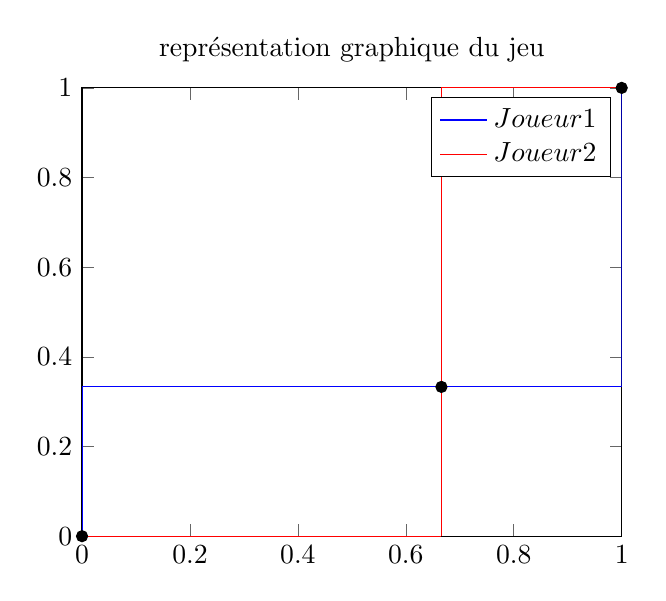
\begin{tikzpicture}
\begin{axis}[
	xmin=0, xmax=1, ymin=0, ymax=1, title={représentation graphique du jeu}
	]
    \addplot [color=blue] coordinates { (0,0)(0,0.333) };
    \addplot [color=red] coordinates { (0,0)(0.666,0) };
    \addplot [color=blue] coordinates { (0,0.333)(1,0.333) };
    \addplot [color=blue] coordinates { (1,0.333)(1,1) };
    \addlegendentry{$Joueur 1$}
    \addplot [color=red] coordinates { (0.666,0)(0.666,1) };
    \addplot [color=red] coordinates { (0.666,1)(1,1) };
    \addlegendentry{$Joueur 2$}
    \addplot [only marks, mark=*, color=black] coordinates { (0,0) (1,1) (0.666,0.333) };
\end{axis}
\end{tikzpicture}

\pagebreak
\subsection{Coopération}

\begin{tabular}{c|cc}
$ $ & f & c\\
\hline
f & 2,1 & 0,0\\
c & 0,0 & 1,2\\
\end{tabular}

Que se passe t'il si les 2 joueurs peuvent communiquer avant de jouer?:
\formula{$u_1 = u_2 = \frac{1}{2} * 2 + \frac{1}{2} = \frac{3}{2}$}

Lorsque tout les joueurs peuvent observer un même événement aléatoire, ils peuvent alors s'accorder sur des équilibres corrélés.\\
Selon un accord prit via un flip coin, ou via une parution d'un évènement, si les deux joueurs se mette d'accord sur le fait de tirer $f$ ou $c$, mais le joueur désavantagé peut ne pas jouer le choix prit, mais il s'expose à ne rien gagner.\\

\subsection{Itération le dilemme des prisonniers}
Deux personne sont arrêtées ensemble en possession d'armes à feu sont soupçonnés d'un délit fait en commun, Les policiers les séparent et disent à chacun:
\begin{description}
\item[] Si l'un des deux avoue et que l'autre ne dit rien, le premier est libéré et le second emprisonné 5 ans.
\item[] Si les deux avouent, les deux iront 4 ans en prison.
\item[] Si les deux ne disent rien alors ils seront emprisonné 2 ans.
\end{description}

Donnant le tableau suivant:
\begin{tabular}{c|cc}
$ $ & P2 avoue & P2 rien\\
\hline
P1 avoue & 4,4 & 0,5\\
P1 rien  & 5,0 & 2,2\\
\end{tabular}

\ \\
Mais les valeurs inscrit ne représente pas le gain, donc il faut inverser les valeurs par rapport au maximum ($5$):\\

\begin{tabular}{c|cc}
$ $ & P2 avoue & P2 rien\\
\hline
P1 avoue & 1,1 & 5,0\\
P1 rien  & 0,5 & 3,3\\
\end{tabular}

Si le joueur 1 avoue et le joueur 2 ne dit rien alors le joueur 1 gagnera 5 ans et le joueur 2 gagner 0 ans (car il sera en prison).\\

\subsection{DIP Itérations}

\begin{description}
\item[] Les joueurs se rencontrent plusieurs fois
\item[] A chaque itération les joueurs ont connaissances des coups précédents 
\item[] ils ne connaissent pas les terme du jeu
\item[] le gain d'un joueur est le cumul des gains de chaque rencontre
\item[] Pour favoriser le coopération on ajoute la contrainte \formula{$X + T < 2R$}
\end{description}
\scalebox{0.8}{
\begin{tabular}{c|cc}
$ $ & Coopérer & non coopérer\\
\hline
Coopérer & $R=3$ récompense pour coopération mutuelle & $S=0$ salaire de la dupe\\
non coopérer & $T=5$ tentation à trahir & $P=1$ punition pour la trahison mutuelle\\
\end{tabular}}

\subsection{Les Stratégies}

Dans une rencontre les joueurs peuvent avoir plusieurs comportements diffèrent, appliquons les sur le problème DIP:
\begin{description}
\item[gentille] le joueur sera gentil quitte à perdre
\item[méchante] le joueur ne laisse rien passé, tout doit être acquérir 
\item[par pattern] suivre la même séquence de choix à l'infini
\item[rancunière] donnant donnant jusqu'à l'erreur de l'adversaire
\item[lunatique] aléatoirement
\item[majoritaire gentille] joue ce que l'autre joue
\item[majoritaire méchante] trahir
\item[donnant donnant] joue le coup précédent de l'autre
\end{description}

Quand on fait jouer ses stratégies dans le cadre d'un tournois on obtient les scores suivant:

\begin{center}
\begin{tabular}{c|cc}
place & stratégie & points \\
\hline
1 & donnant donnant & 42 \\
2 & majoritaire gentille & 19 \\
3 & rancunière & 4\\
4 & lunatique  & 0\\
\end{tabular}
\end{center}
\ \\
le top 3 n'est pas compliqué à déduire, se sont tous des stratégies adaptatif (qui s'adapte à l'adversaire).\\
le top 2 a un pouvoir pour pardonner l'adversaire donc un jugement moins punitif.\\
le top 1 est simple, il incarne la simplicité.\\
la gentillesse prime aussi.\\

\pagebreak
\section{Jeux répété}

Soit un jeu $G = \{S, \{u_i \} i=1,...n \}$ où $S$ est l'ensemble fini des profils stratégie et $u_i$ est la fonction d'utilité du joueur $i$.\\
On note $(G,T)$ le jeu répété obtenu en jouant $T$ fois le jeu de base $G$, $(G,\infty)$ correspond à un nombre infini de tour.\\

On peut également distinguer les jeux répété un nombre fini, mais indéfini de fois : à chaque tour, il y a une probabilité $1 - q$ 
que le jeu s'arrête.\\
Facteur d'actualisation: Lorsqu'un jeu est répété, il se peut que les gains obtenus à l'itération courante $u_t$ soient plus/moins importants aux yeux de l'agent que les gains  l'itération suivante $u_{t+1}$. Pour modéliser cela on peut utiliser un facteur d'actualisation $\phi$:
\formula{$u_t = \phi u_{t+1}$}

Le facteur d'actualisation $\phi = \frac{u_t}{u_{t+1}}$ représente donc l'attrait du joueur pour les gains actuels.

\subsection{Jeux à deux joueurs à somme nulle}

Dans le cas d'un jeu à somme nulle pour chaque case le joueur 1 va gagner la somme indiqué et le joueur 2 va perdre la somme indiqué:\\
\begin{center}
\begin{tabular}{c|cccc}
$ $ & $y_1$ & $y_2$ & $y_3$ & $y_4$ \\
\hline
$x_1$ & 18 & 3 & 0 & 2\\
$x_2$ & 0 & 3 & 8 & 20\\
$x_3$ & 5 & 4 & 5 & 5\\
$x_4$ & 9 & 3 & 0 & 20\\
\end{tabular}
\end{center}
\ \\
si le joueur 1 prend $x_1$ et le joueur 2 $y_1$ alors le joueur 1 gagnera 18 et le joueur 2 perdra 18.\\

Le joueur 1 tente de maximiser son niveau de sécurité:
\formula{$v_x = max_i(min_j u(x_i,y_j))$}

Le joueur 2 tente de minimiser le niveau de sécurité du joueur 1:
\formula{$v_y = min_j(max_i u(x_i,y_j))$}

\subsection{Jeu sous forme extensive}

Un jeu se déroulant de la racine jusqu'à une feuille, le noeud indique quel joueur doit jouer, donc un ordre de passage est explicite.\\

Soit le jeu suivant sous forme d'arbre:

\begin{center}
\scalebox{0.8}{
\begin{tikzpicture}[->,>=stealth',shorten >=1pt,auto,node distance=3cm,
                    semithick]
  \tikzstyle{every state}=[fill=white,draw=none,text=black]

  \node[initial, state](A)                    {$1$};
  \node[state]         (B) [below of=A]       {$2$};
  \node[state]         (C) [right of=A]       {$3$};
  \node[state]		   (D) [right of=C]       {$(3,2,2)$};
  \node[state]         (AA)[below left of=A]  {$(3,0,0)$};
  \node[state]         (BA)[below left of=B]  {$(4,2,4)$};
  \node[state]		   (BB)[below right of=B] {$(2,3,1)$};
  \node[state]    	   (CA)[below  of=C]      {$(1,0,3)$};

  \path (A) edge 			  node {x} (AA)
  			edge			  node {y} (B)
  		    edge 			  node {z} (C)
  		(B) edge 			  node {w'} (BA)
  		    edge 			  node {u'} (BB)
  		(C) edge              node {u}  (CA)
  		    edge 			  node {w}  (D);
\end{tikzpicture}
}\end{center}

\begin{multicols}{2}
[Via la récurrence à rebours, On remonte les noeuds optimaux de l'arbre vers la racine:]
\scalebox{0.7}{
\begin{tikzpicture}[->,>=stealth',shorten >=1pt,auto,node distance=3cm,semithick]
  \tikzstyle{every state}=[fill=white,draw=none,text=black]

  \node[initial, state](A)                    {$1$};
  \node[state]         (B) [below of=A]       {$(2,3,1)$};
  \node[state]         (C) [right of=A]       {$(1,0,3)$};
  \node[state]         (AA)[below left of=A]  {$(3,0,0)$};

  \path (A) edge 			  node {x} (AA)
  			edge			  node {y} (B)
  		    edge 			  node {z} (C);
\end{tikzpicture}
}
\scalebox{0.7}{
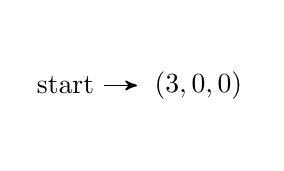
\begin{tikzpicture}[->,>=stealth',shorten >=1pt,auto,node distance=3cm,semithick]
  \tikzstyle{every state}=[fill=white,draw=none,text=black]

  \node[initial, state](A)                    {$(3,0,0)$};

\end{tikzpicture}
}
\end{multicols}

\subsection{sous jeu}
Un sous jeu d'un jeu sous forme extensive est un jeu composé d'un noeud (qui est un ensemble d'information singleton) de tous les noeuds successeurs de ce noeud, de tout les arcs reliant ces noeuds, et des unités associées à tout les noueds terminaux successeurs.
\\
Le grand arbre ci dessus contient 3 sous jeux ayant comme racine (1,2,3).\\

\pagebreak
\subsection{Menaces non crédibles}

\begin{multicols}{2}
[Voici le même jeu sous forme de tableau et sous forme d'arbre]
\scalebox{0.65}{
\begin{tikzpicture}[->,>=stealth',shorten >=1pt,auto,node distance=3cm,semithick]
  \tikzstyle{every state}=[fill=white,draw=none,text=black]

  \node[initial, state](A)                    {$1$};
  \node[state]         (B) [below of=A]       {$2$};
  \node[state]         (AA)[below left of=A]  {$(2,2)$};
  \node[state]         (BA)[below left of=B]  {$\crouge{(3,1)}$};
  \node[state]		   (BB)[below right of=B] {$(0,0)$};

  \path (A) edge 			  node {x} (AA)
  			edge			  node {y} (B)
  		(B) edge 			  node {u} (BA)
  		    edge 			  node {v} (BB);
\end{tikzpicture}
}

\begin{tabular}{c|cc}
$ $ & u & v\\
\hline
x & (2,2) & $\crouge{(2,2)}$\\
y & $\crouge{(3,1)}$ & (0,0)\\
\end{tabular}
\end{multicols}

L'équilibre de Nash de l'arbre indique que la meilleur stratégie (d'un point de vue rationnel) est $(3,1)$ et via le tableau on obtient $\{(3,1),(2,2)\}$.\\
l'équilibre de Nash $(xv)$ n'est pas crédible car il repose sur la menace non-crédible du joueur 2 de joueur $v$, autrement dit, dans le premier tour, si le joueur 1 joue $x$, le joueur 2 n'a aucun choix à faire, hors dans le tableau le joueur 2 peut proposer un choix.\\

Un équilibre de Nash d'un jeu sous forme extensive est un équilibre parfait en sous jeu si toute restriction du profil de stratégies à un sous jeu est un équilibre de Nash pour ce sous jeu.\\
Pour les jeux à informations parfaites, la notion d'équilibre parfait en sous jeu coïncide avec la notion de récurrence à rebours.\\ 

\pagebreak
\subsection{Promesse non crédible}
Soit un contrat pour travailler en entreprise, le joueur 2 étant vous et le joueur 1 étant l'entreprise:

\begin{center}
\scalebox{0.7}{
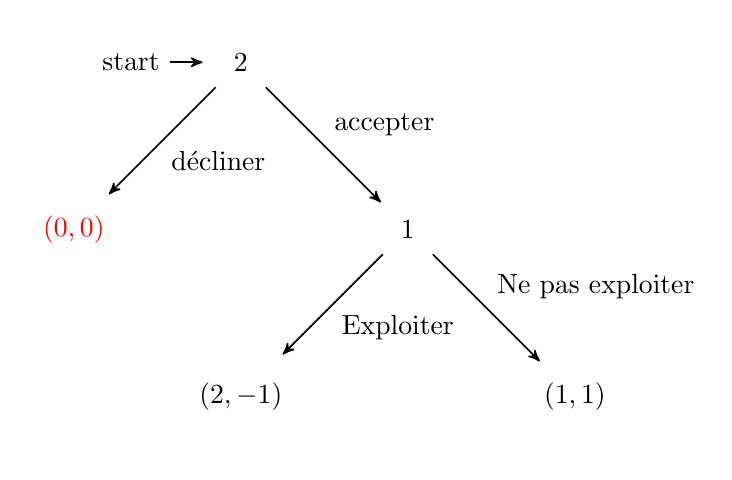
\begin{tikzpicture}[->,>=stealth',shorten >=1pt,auto,node distance=3cm,semithick]
  \tikzstyle{every state}=[fill=white,draw=none,text=black]

  \node[initial, state](A)                    {$2$};
  \node[state]         (B) [below right of=A] {$1$};
  \node[state]         (AA)[below left of=A]  {$\crouge{(0,0)}$};
  \node[state]         (BA)[below left of=B]  {$(2,-1)$};
  \node[state]		   (BB)[below right of=B] {$(1,1)$};

  \path (A) edge 			  node {décliner} (AA)
  			edge			  node {accepter} (B)
  		(B) edge 			  node {Exploiter} (BA)
  		    edge 			  node {Ne pas exploiter} (BB);
\end{tikzpicture}
}
\end{center}
Dans le cas d'un contrat non répété il est mieux de choisir $\crouge{(0,0)}$, mais dans le cas d'un jeu répété si vous êtes le premier candidat et que vous acceptez le poste mais que vous vous faite exploiter, alors vous aller altérer les nouveaux candidats pour qu'ils choisis l'option de ne pas aller travailler la bas, donc l'entreprise ne devrait pas vous exploiter pour son bien.\\

\subsection{Limite de la récurrence à rebours}

Soit le jeu suivant, vous êtes le joueur 1:
\begin{center}
\scalebox{0.6}{
\begin{tikzpicture}[->,>=stealth',shorten >=1pt,auto,node distance=3cm,semithick]
  \tikzstyle{every state}=[fill=white,draw=none,text=black]

  \node[initial, state](A)                    {$1$};
  \node[state]         (B) [right of=A]       {$2$};
  \node[state]         (C) [right of=B]       {$1$};
  \node[state]         (D) [right of=C]       {$2$};
  \node[state]         (AA)[below of=A]       {$\crouge{(98,98)}$};
  \node[state]         (BA)[below of=B]       {$(97,100)$};
  \node[state]         (CA)[below of=C]       {$(99,99)$};
  \node[state]         (DA)[below of=D]       {$(98,101)$};
  \node[state]         (DB)[right of=D]       {$(100,100)$};

  \path (A) edge 			  node {D} (AA)
  			edge			  node {R} (B)
  		(B) edge 			  node {D} (BA)
  		    edge 			  node {R} (C)
  		(C) edge              node {D} (CA)
  		    edge              node {R} (D)
  		(D) edge              node {D} (DA)
  		    edge 			  node {R} (DB);
\end{tikzpicture}
}
\end{center}
Le calcule de l'équilibre de Nash nous donne $\crouge{(98,98)}$ mais cette équilibre ne marche que si le joueur 2 est un robot / rationnel, si on indique que les somme sont des Millions d'euro, les choix seront bien plus différent, si les deux joueurs sont altruiste alors les deux vont gagner $(100,100)$ si l'un des joueur est mauvais alors celui ci va aller le plus haut possible et choisir $D$ juste en guise de dernier choix.\\

\pagebreak
\section{Jeux coopératifs à 2 joueurs}

%% fill

\pagebreak
\chapter{Décision de groupe et théorie du vote}
Soit un ensemble de candidats $X = \{a,b,c....\}$, un sous ensemble de $X$ est noté un agenda.\\
Soit une relation d'ordre $<, >$ (réflexif, transitif, total) permettent de trier les éléments de X selon des critères.\\
Un ensemble d'individu est appelé un profil, chaque individu a le même poids.\\
\\
On n'aura deux façon de procéder:
\begin{description}
\item[] Déterminer la relation de préférence (l'ordre des candidats).
\item[] Déterminer le gagnant d'un vote. (faisable aussi via la première façon). 
\end{description}
\pagebreak

\section{Vote entre 2 candidats}
$A > B$ si le nombre d'individu qui préfèrent A et plus grande que le nombre d'individu qui préfèrent B.\\

Quatre propriété:
\begin{description}
\item[Domaine universel] la méthode de vote donne un résultat quel que soit le profil.
\item[Anonymat] La méthode de vote traite tout les votant de la même manière.
\item[Neutralité] La méthode de vote traite tous les candidats de la me manière.
\item[Monotonie] Si un candidat est élu pour un profil donné, il sera forcément élu pour un profil modifié où ce candidat reçoit plus de vote.
\end{description}
\ \\

\section{Gagnant de Condorcet}
\begin{multicols}{2}
[Un gagnant de Condorcet $A$ et un profil N si pour tout autre candidat $B \in$ N, le candidat $A$ est majoritairement préféré à $B$.
]
\begin{description}
\item[] $a >_1 b >_1 c$
\item[] $a >_2 c >_2 b$
\item[] $c >_3 b >_3 a$
\end{description}
\begin{description}
\item[] Pour X = \{a,b\} a = 2, b = 1
\item[] Pour X = \{a,c\} a = 2, c = 1
\item[] a est un gagnant de Condorcet
\end{description}
\end{multicols}

\begin{multicols}{2}
[
Pour tout les profil, il existe qu'un gagnant, mais il peut en avoir aucun:]
\begin{description}
\item[] $a >_1 b >_1 c$
\item[] $b >_2 c >_2 a$
\item[] $c >_3 a >_3 b$
\end{description}
\begin{description}
\item[] Pour X = \{a,b\} a = 2, b = 1
\item[] Pour X = \{a,c\} a = 1, c = 2
\item[] Pour X = \{b,c\} b = 2, c = 1
\end{description}
\end{multicols}

Une méthode de choisir le gagnant de Condorcet quand il existe est appelée Condorcet cohérente.

\section{Scrutin majoritaire simple}

\begin{multicols}{2}
[Adapter le vote entre 2 candidats, soit 21 votants:]
\begin{description}
\item[10:] $a >_1 b >_1 c$
\item[6:] $b >_2 c >_2 a$
\item[5:] $c >_3 b >_3 a$
\end{description}
\begin{description}
\item[] Résultat: a 10, b 6, c 5
\item[] Le candidat a est élu
\item[] 
\end{description}
\end{multicols}

Mais le problème et que plus de vote sont en faveur de $b$ que de $a$, on parle de perdant de Condorcet (ou de vote pour le pire candidat).

\section{Scrutin majoritaire à deux tour}
\begin{multicols}{2}
[Hors majorité absolu, le vote se fera via un scrutin à 2 tours:]
\begin{description}
\item[10:] $a >_1 b >_1 c$
\item[6:] $b >_2 c >_2 a$
\item[5:] $c >_3 b >_3 a$
\end{description}
\begin{description}
\item[] Premier tour: a 10, b 6, c 5, le candidat c est éliminé
\item[] Second tour : a 10, b 11
\item[] Le candidat b est élu
\end{description}
\end{multicols}

Le scrutin majoritaire à deux tours est manipulable, il peut être profitable à un individu de mentir sur ses préférences.\\
Le scrutin majoritaire à deux tours est non-monotone et n'incite pas à la participation.\\
Le scrutin majoritaire à deux tours n'est pas séparable. l'union de ce même vote via deux circonscriptions différente ayant comme élu le même candidat ne garantit pas que ce même candidat sera élu lors de la fusion des circonscriptions.\\
Le scrutin majoritaire à deux tours permet la dictature de la majorité, si dans deux circonscriptions:
\begin{description}
\item[] 51: a > b > c ... > z
\item[] 49: z > b > c ... > a
\end{description}
Le candidat a gagne via utilisation de la règle de dictature alors que le candidat b a 100\% de vote sur le second choix de préférence.\\

\section{Méthode de vote non rangées}

% fill

\section{Méthode par scorage}

% fill like ROC

\section{Méthode de Condorcet cohérentes}

% fill Coperland
% fill Kramer Simpson
% règle de tile break

\section{Graphe de majorité}

% fill
% gagnant de condocet a toute les fléches sortante

\pagebreak
\part{Apprentissage}
\pagebreak

\chapter{Approche d'apprentissage par la logique}
Une approche simple concernant l'apprentissage de problèmes dont le domaine de sortie est boolean
serait de passer par la logique classique pour pouvoir simplifier la compréhension du problème.\\
\pagebreak
\section{Espace de Version}
Pour un problème suivant:

$\begin{tabular}{cccc|c}
\hline
A & B & C & D & accaptable? \\
\hline
1 & 1 & 1 & 0 & oui\\
1 & 1 & 0 & 1 & oui\\
0 & 1 & 1 & 1 & non\\
\hline
\end{tabular}$

\ \\
D'où il suffirait d'une fonction donnant dans le domaine Boolean, associer un algorithme de classification simple:\\
\ \\
\vspace{1cm}
\scalebox{0.7}{
\begin{tikzpicture}
  \begin{axis} [
      xlabel     = X, % label x axis
      ylabel     = Y, % label y axis
      axis lines = left, %set the position of the axes
      clip       = false, 
      xmin       = 0,
      ymin       = 0,
    ]
    \addplot [color=black] coordinates { (0,0)(5,5) };
    \addplot [only marks, mark=*, color=blue] coordinates {(1,4)(3,3.5) };
    \addplot [only marks, mark=*, color=red] coordinates {(4,2) };
  \end{axis}
\end{tikzpicture}
}

\vspace{1cm}

Ayant comme points de couleurs $\crouge{Rouge}$ les points donnant la valeur de vérité False et les points de couleurs $\cblue{Blue}$ les point donnant la valeur de vérité True.\\
Mais ce ne serait pas donner un gros mode de résolution à un problème qui peut être simplifié?\\
\\
Pour les cas suivants:
\begin{description}
\item[-] Faciliter la compréhension du problème
\item[-] Comprendre pourquoi une décision donné pour une entrée
\end{description}
\pagebreak

\subsection{convergence des données}

Dans le tableau d'acceptation on peut transformé la règle 3 en son dual via la Lois de De Morgan:\\

\begin{multicols}{2}
[Et via un treillis de donnée pour chaque entré positif on peut compter le nombre d'occurrence de motif en faveur de l'acceptation de la ligne:]
\scalebox{0.3}{
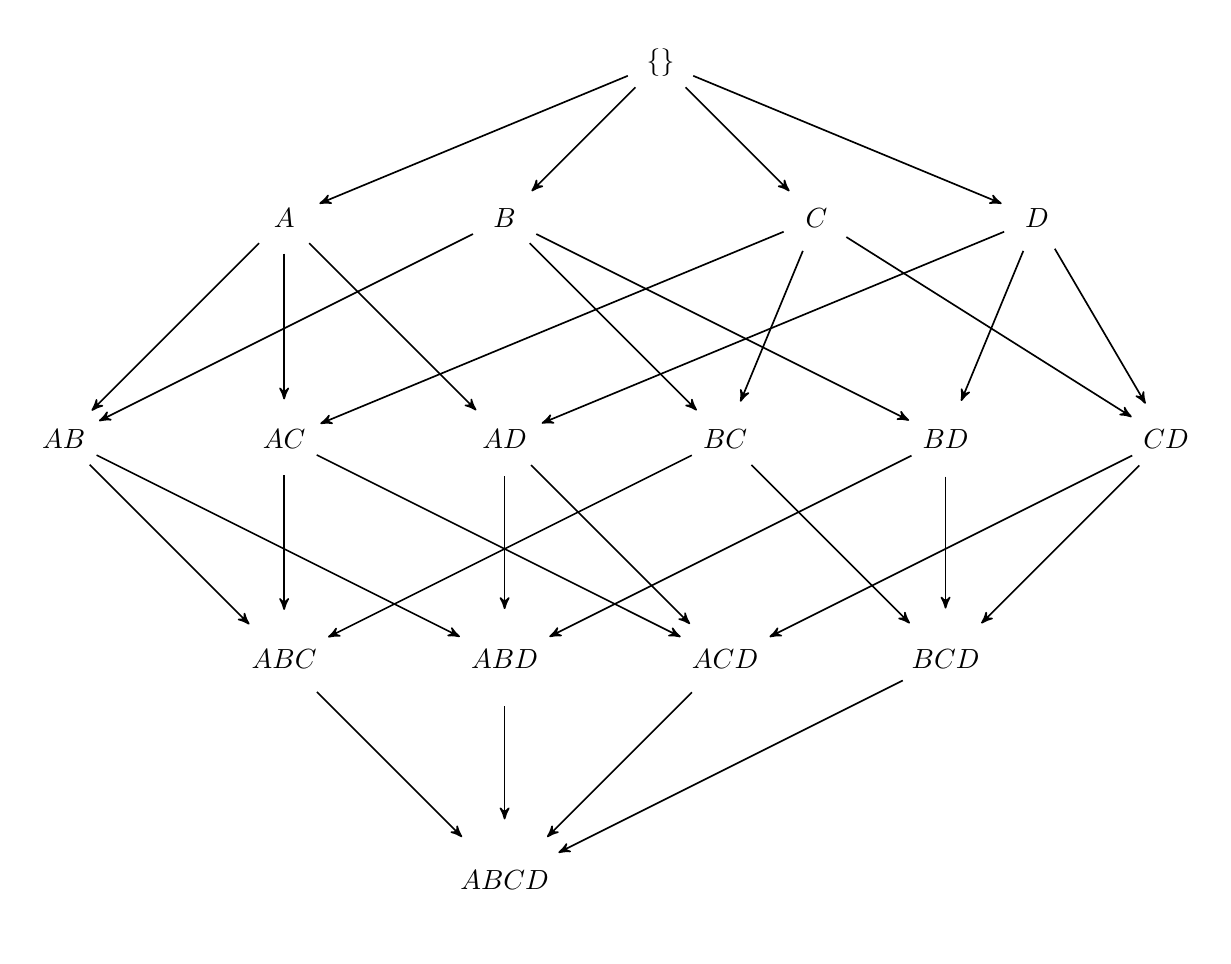
\begin{tikzpicture}[->,>=stealth',shorten >=1pt,auto,node distance=2.8cm,
                    semithick]
  \tikzstyle{every state}=[fill=white,draw=none,text=black]

  \node[state]         (Z)                    {$\{\}$};
  \node[state]         (B) [below left  of=Z] {$B$};
  \node[state]         (A) [left  of=B]       {$A$};
  \node[state]         (C) [below right of=Z] {$C$};
  \node[state]         (D) [right of=C]       {$D$};
  \node[state]		   (AC) [below  of=A]     {$AC$};
  \node[state]		   (AB) [left of=AC]      {$AB$};
  \node[state]		   (AD) [right of=AC]     {$AD$};
  \node[state]         (BC) [right of=AD]     {$BC$};
  \node[state]		   (BD) [right of=BC]	  {$BD$};
  \node[state]		   (CD) [right of=BD] 	  {$CD$};
  \node[state]		   (ABD) [below of=AD]    {$ABD$};
  \node[state] 		   (ABC) [left of=ABD]    {$ABC$};
  \node[state]		   (ACD) [right of=ABD]   {$ACD$};
  \node[state]		   (BCD) [right of=ACD]   {$BCD$};
  \node[state]	       (ABCD) [below of=ABD]  {$ABCD$};
  

  \path (Z) edge              node {} (A)
            edge              node {} (B)
            edge			  node {} (C)
            edge  			  node {} (D)
        (A) edge			  node {} (AB)
        	edge			  node {} (AC)
        	edge			  node {} (AD)
        (B) edge			  node {} (AB)
        	edge			  node {} (BC)
        	edge 			  node {} (BD)
        (C) edge 			  node {} (AC)
        	edge			  node {} (BC)
        	edge 			  node {} (CD)
        (D) edge 			  node {} (AD)
        	edge 			  node {} (BD)
        	edge 			  node {} (CD)
        (AB) edge 			  node {} (ABC)
        	edge 			  node {} (ABD)
        (AC) edge			  node {} (ABC)
        	edge 			  node {} (ACD)
        (AD) edge 			  node {} (ABD)
        	edge			  node {} (ACD)
        (BC) edge			  node {} (ABC)
        	edge  			  node {} (BCD)
        (BD) edge			  node {} (ABD)
        	edge 			  node {} (BCD)
        (CD) edge 			  node {} (ACD)
        	edge			  node {} (BCD)
        (ABC) edge 			  node {} (ABCD)
        (ACD) edge 			  node {} (ABCD)
        (ABD) edge 			  node {} (ABCD)
        (BCD) edge 			  node {} (ABCD);
\end{tikzpicture}
}
$\begin{tabular}{cccc|c}
\hline
A & B & C & D & accaptable? \\
\hline
1 & 1 & 1 & 0 & oui\\
1 & 1 & 0 & 1 & oui\\
1 & 0 & 0 & 0 & oui\\
\hline
\end{tabular}$
\end{multicols}
\ \\

\begin{multicols}{2}
[]
\scalebox{0.4}{
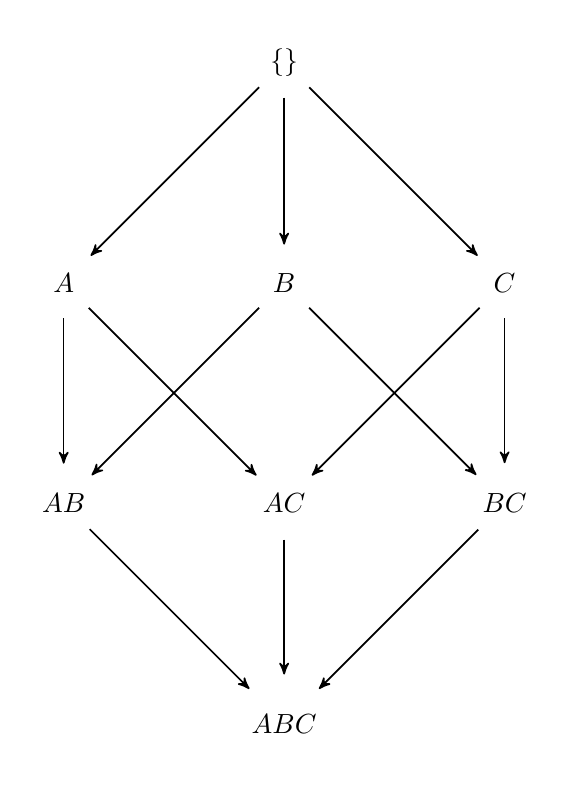
\begin{tikzpicture}[->,>=stealth',shorten >=1pt,auto,node distance=2.8cm,
                    semithick]
  \tikzstyle{every state}=[fill=white,draw=none,text=black]

  \node[state]         (Z)                    {$\{\}$};
  \node[state]         (B) [below  of=Z]      {$B$};
  \node[state]         (A) [left  of=B]       {$A$};
  \node[state]         (C) [right of=B]       {$C$};
  \node[state]		   (AB) [below of=A]      {$AB$};
  \node[state]		   (AC) [right of=AB]     {$AC$};
  \node[state]         (BC) [right of=AC]     {$BC$};
  \node[state] 		   (ABC) [below of=AC]    {$ABC$};
  

  \path (Z) edge              node {} (A)
            edge              node {} (B)
            edge			  node {} (C)
        (A) edge			  node {} (AB)
        	edge			  node {} (AC)
        (B) edge			  node {} (AB)
        	edge			  node {} (BC)
        (C) edge 			  node {} (AC)
        	edge			  node {} (BC)
        (AB) edge 			  node {} (ABC)
        (AC) edge			  node {} (ABC)
        (BC) edge			  node {} (ABC);
\end{tikzpicture}
}
$\begin{tabular}{cccc|c}
\hline
A & B & C & D & accaptable? \\
\hline
\crouge{1} & \crouge{1} & \crouge{1} & \crouge{0} & \crouge{oui}\\
1 & 1 & 0 & 1 & oui\\
1 & 0 & 0 & 0 & oui\\
\hline
\end{tabular}$
\end{multicols}
\pagebreak

\begin{multicols}{2}
[]
\scalebox{0.4}{
\begin{tikzpicture}[->,>=stealth',shorten >=1pt,auto,node distance=2.8cm,
                    semithick]
  \tikzstyle{every state}=[fill=white,draw=none,text=black]

  \node[state]         (Z)                    {$\{\}$};
  \node[state]         (B) [below  of=Z]      {$B$};
  \node[state]         (A) [left  of=B]       {$A$};
  \node[state]		   (AB) [below of=A]      {$AB$};
  

  \path (Z) edge              node {} (A)
            edge              node {} (B)
        (A) edge			  node {} (AB)
        (B) edge			  node {} (AB);
\end{tikzpicture}
}
$\begin{tabular}{cccc|c}
\hline
A & B & C & D & accaptable? \\
\hline
1 & 1 & 1 & 0 & oui\\
\crouge{1} & \crouge{1} & \crouge{0} & \crouge{1} & \crouge{oui}\\
1 & 0 & 0 & 0 & oui\\
\hline
\end{tabular}$
\end{multicols}

\begin{multicols}{2}
[]
\scalebox{0.4}{
\begin{tikzpicture}[->,>=stealth',shorten >=1pt,auto,node distance=2.8cm,
                    semithick]
  \tikzstyle{every state}=[fill=white,draw=none,text=black]

  \node[state]         (Z)                    {$\{\}$};
  \node[state]         (A) [left  of=B]       {$A$};
  

  \path (Z) edge              node {} (A);
\end{tikzpicture}
}
$\begin{tabular}{cccc|c}
\hline
A & B & C & D & accaptable? \\
\hline
1 & 1 & 1 & 0 & oui\\
1 & 1 & 0 & 1 & oui\\
\crouge{1} & \crouge{0} & \crouge{0} & \crouge{0} & \crouge{oui}\\
\hline
\end{tabular}$
\end{multicols}

\ \\
Par itération et réduction du treillis on sait que $A$ et un attribut très discriminant, qui fait revenir le problème à seulement la valeur de $A$.\\

\pagebreak
\chapter{Apprentissage statistique}

Dans ce chapitre nous nous intéressons à des fonctions $h \in H$ à qui pour une liste $X$ à $d$ dimension de domaine réelle associe un label $y$ dans le domaine $[-1,+1]$. Un $x \in X$ peut être une couleur, un réelle, une chose négatif ou encore une mesure quelconque.
\pagebreak

\section{Classification binaire réalisable}

Chaque entrée $x \in X$ est tirée aléatoirement et indépendamment selon une distribution de probabilité $d$ qui est fixée mais inconnue de l'apprenant.
\\
Chaque sortie $y \in Y$ est calculé via la fonction cible $h* \in H$ qui est inconnue de l'apprenant.

\subsection{Erreur de généralisation et d'entrainement}

La performance d'une hypothèse $h \in H$ est calculé par le nombre d'erreurs que la fonction peut commettre en probabilité selon $d$:
\begin{description}
\item[] $l_d(h)$ = $P_{x~d}[h(x) \neq h*(x)]$
\end{description}

En pratique, l'apprenant n'a accès qu'a une petite partit nommé $S \in X$ (qui peut contenir des doublons) dont les éléments dont générés aléatoirement via $d$, Le risque empirique de $h$ par rapport à $S$ est donné par :
\begin{description}
\item[] $l_s(h)$ = $\frac{1}{|S|} |\{x \in S : h(x) \neq h*(x)\}|$
\end{description}
Le nombre d'erreur moyen que fait $h$ sur $S$\\

\subsection{Processus d'apprentissage}

Le processus d'apprentissage n'est pas si différent que dans la première partie du Memo:\\

Soit une distribution $d$, chaque requêtes vers $d$ va choisir un échantillons aléatoirement pour crée un ensemble $S$ qui va servir à faire apprendre $h$ lors de la phase d'apprentissage, tester lors de la phase de teste et retenir les erreur vies les fonction d'analyse.\\

\subsection{Incertitude de l'apprentissage}

Il existe deux mesures de l'incertitude en apprentissage statistique
\begin{description}
\item[] Paramètre de confiance qui donne la qualité de l'échantillonnage
\item[] Paramètre d'erreur qui donne un indice sur les bonnes prédictions futures
\end{description}

\subsection{Modèle PAC réalisable}
Une classe d(hypothèses $H$ est dite PCA (probability approximately correct) s'il existe une fonction $\{0,1\}^2 \rightarrow \{0,1,2.....\}$ telle que pour toute paire ($\phi$(confiance),$\psi$(erreur)) pour toute distribution $d$ sur $X$ et toute fonction cible $h* \in H$:
\begin{description}
\item[] Après avoir observé un échantillon $S$ de $X$ tiré aléatoirement selon $d$, et de taille au moins $m(\phi,\psi)$.
\item[] L'apprenant retourne une hypothèse $h \in H$, telle qu'avec une probabilité au moins $1 - \phi$, l'erreur de génération $l_d(h)$ est d'au plus $\psi$.
\end{description}

\section{Classes d'hypothèses finies}

Supposons $X$ = $[0,1]^d$

\begin{description}
\item[] Toutes fonction $h: [0,1]^d \rightarrow [0,1]$ est appelée fonction booléenne.
\item[] Une classe d'hypothèses booléennes est un sous ensemble $H$ de $[[0,1]^d \rightarrow [0,1]]$.
\end{description}

\subsection{Minimisation des erreurs empirique}
Le principe est de trouver dans $H$ l'hypothèse qui fait le moins d'erreurs sur l'échantillon $S$:
\formula{$h_S \in argmin L_S(h), h \in H$}


\subsection{Théorème de PAC des classes finies}
Toutes classe d'hypothèse $H$ finie est PAC-apprenable avec une complexité d'échantillonnage
\formula{$m(\phi,\psi) \leq \frac{ln(|H|/\phi)}{\psi}$}

\pagebreak
\section{Classification binaire agnostique}
\subsection{Régression agnostique}

\pagebreak
\chapter{Apprentissage Online}

L'apprentissage online est un jeu à somme nulle répétitif à deux joueur (théorème minmax ou équilibre de Nash), les joueurs sont l'environnement et le joueur.\\
L'apprenant reçoit une observation de l'environnement et donne une prédiction, et l'environnement va donner la vérification sur la prédiction.\\

\pagebreak
\section{Analyse convexe}
\subsection{Combinaison convexe}

Une forme convexe est une forme pour qui n'importe quel droite dont les 2 points font partie de la forme est dans la forme.\\

\begin{center}

\begin{tikzpicture}[scale=2]
    \matrix[nodes={draw, ultra thick, fill=blue!20},
        row sep=0.3cm,column sep=0.5cm] {

    \node[ellipse] {$Convexe$};&
    \node[star,star points=5, scale=0.5] {$Non\ convexe$};\\
    };
\end{tikzpicture}
\end{center}

\subsection{Enveloppe convexe}

L'enveloppe convexe d'une forme est la bordure\\
\begin{center}
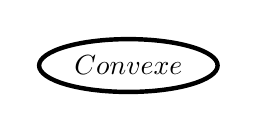
\begin{tikzpicture}[scale=2]
    \matrix[nodes={draw, ultra thick, fill=white},
        row sep=0.3cm,column sep=0.5cm] {

    \node[ellipse] {$Convexe$};\\
    };
\end{tikzpicture}
\end{center}

Si un espace d'application est convexe alors le problème est polynomial, sinon le problème est NP-complet.\\

\cshape{1}{
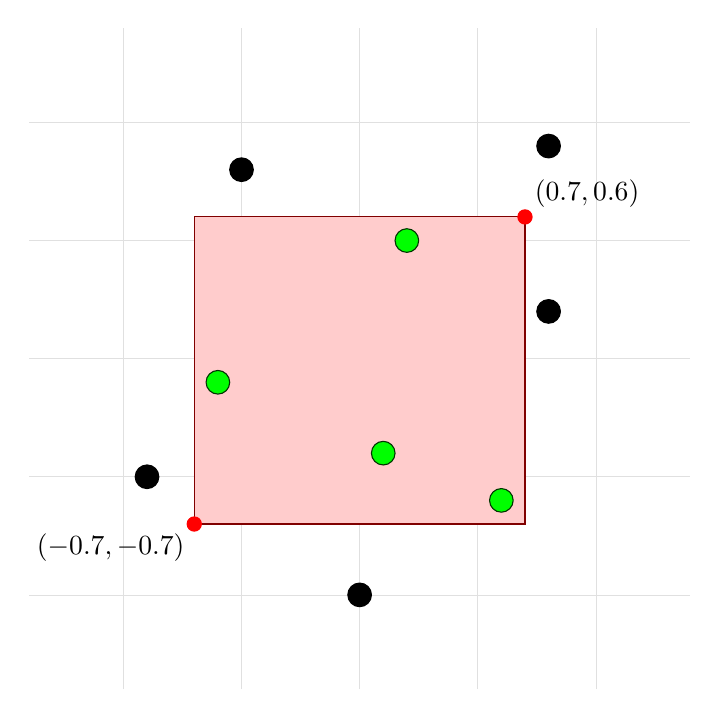
\begin{tikzpicture}[scale=3]
	\draw[step=.5cm,gray!20,very thin] (-1.4,-1.4) grid (1.4,1.4);
	\filldraw[fill=red!20!white, draw=red!50!black] (-0.7,-0.7) rectangle (0.7,0.6);
	
	\foreach \coord in {(-0.5,0.8),(0.8,0.2),(-0.9,-0.5),(0,-1),(0.8,0.9)}{
		\draw[fill=black, draw=black] \coord circle (0.05cm);
	}
	
	\foreach \coord in {(0.2,0.5),(0.1,-0.4),(-0.6,-0.1),(0.6,-0.6)}{
		\draw[fill=green, draw=green!20!black] \coord circle (0.05cm);
	}
	
	\foreach \coord in {(-0.7,-0.7),(0.7,0.6)}{
		\draw[fill=red, draw=red] \coord circle (0.03cm);
	}
	
	\draw (-0.7,-0.7) node[below left] {$(-0.7,-0.7)$};
	\draw (0.7,0.6)   node[above right]{$(0.7,0.6)$};
\end{tikzpicture}
}

Dans cette figure on calcule l'enveloppe en essayant de capturer tout les points vert, un carré de coordonné $(-0.7,-0.7)(0.7,0.6)$ peut largement faire le boulot et résoudre le problème de classification.\\
Le calcule est polynomial (enfin même inférieur) car le calcul de la classification d'un point se fait en un 4 instructions simple:\\
\formula{$classification = \cblue{lambda}\ x,y : -0.7 < x < 0.7\ \cviolet{and}\ -0.7 < y < 0.6$}
Ce raisonnement est valide car il n'y a aucun point noir dans le rectangle rouge.\\

\pagebreak
\subsection{Theoreme de la séparation des hyperplan}

Un hyperplan est un ensemble de points sous la forme (représenté en blue):
\formula{$H = \{x | a^T x = b\}, a \neq 0\ and\ b \in R$}
\ \\
Un hyperespace est un ensemble de points sous le forme (représenté en rouge):
\formula{$H = \{x | a^T x \leq b \}, a \neq 0\ and\ b \in R$}

\cshape{0.8}{
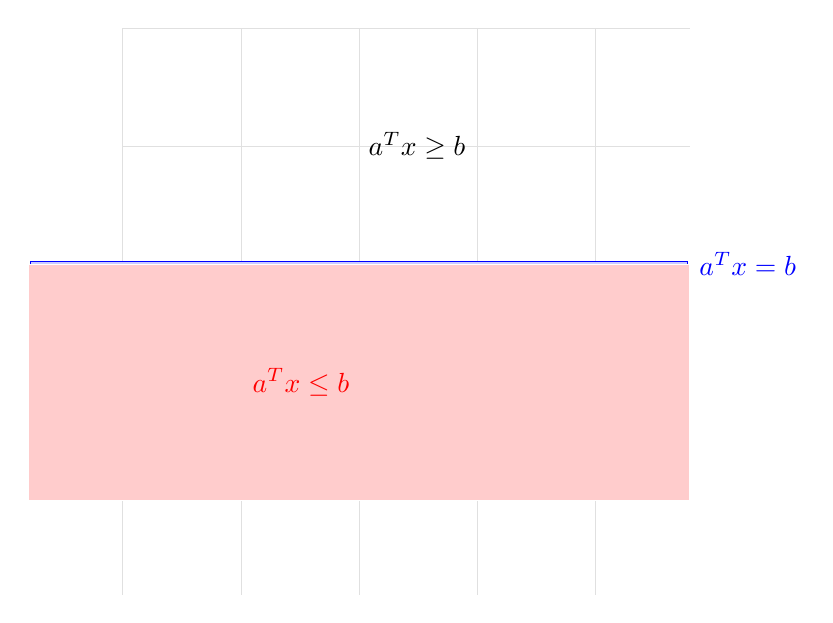
\begin{tikzpicture}[scale=3]
	\draw[step=.5cm,gray!20,very thin] (-1,-1.4) grid (1.4,1);
	\filldraw[fill=blue!20!white, draw=blue!100!black] (-1.39,0.01) rectangle (1.39,-0.01);
	\filldraw[fill=red!20!white, draw=red!0!white] (-1.4,0) rectangle (1.4,-1);
	
	\draw (0,-0.5) node [left] {$\crouge{a^T x \leq b}$};
	\draw (0,0.5)  node [right]{$a^T x \geq b$};
	\draw (1.4,0) node [right] {$\cblue{a^T x = b}$};

\end{tikzpicture}
}
\ \\
Soit $P$ et $N$ deux ensemble de points connexe tel qu'il n'existe aucune intersection, alors il existe une a ($\neq 0$) et un b tel que:
\formula{$a^T x < b \forall x \in P$ and}
\formula{$a^T x \geq b \forall x \in N$}
L'ensemble des $\{x | a^T x = b\}$ est l'hyperplan de séparation de $P$ et $N$.

\cshape{0.6}{
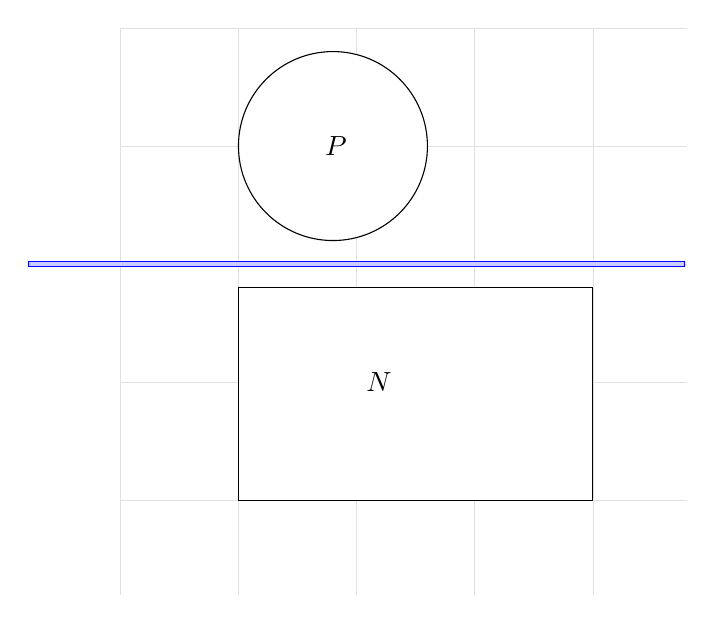
\begin{tikzpicture}[scale=3]
	\draw[step=.5cm,gray!20,very thin] (-1,-1.4) grid (1.4,1);
	\filldraw[fill=white, draw=black] (-0.1,0.5) circle (0.4cm);
	\filldraw[fill=blue!20!white, draw=blue!100!black] (-1.39,0.01) rectangle (1.39,-0.01);
	\filldraw[fill=white, draw=black] (-0.5,-0.1) rectangle (1,-1);
	
	\draw (0,0.5) node [left] {$P$};
	\draw (0,-0.5)  node [right]{$N$};

\end{tikzpicture}
}

\subsection{Gradient}

%% fill

\subsection{Fonction de Perte}

%% fill

\section{Apprentissage par régression}

\section{Apprentissage par classification}

\pagebreak


\part{Problème de satisfaction de contraintes CSP}
\pagebreak

\chapter{Introduction et modèles}
\pagebreak

Une Solution d'un problème CSP est une assignation d'une valeur à chaque variables de P tel que toutes les contraintes de P soit satisfaite.\\

\section{exemple simple}

Trouver une assignation Minimal et Maximal pour chaque variables de P dans le problème suivant:\\
\begin{description}
\item[vars(P)] = $w,x,y,z$
\item[Dom(P)]\  \begin{description}
\item[Dom(w,x)] = $\{1,2,3\}$
\item[Dom(y,z)] = $range(4)$
\end{description}
\item[Contraintes]\  \begin{description}
\item[$~$] $w = x$
\item[$~$] $x \leq y + 1$
\item[$~$] $y > z$
\item[$~$] $(x,z) \in \{(1,2),(2,1),(2,4),(3,3)\}$
\end{description}
\end{description}
\ \\
Une solution serait:
\begin{description}
\item[Minimal] $w=x=1, y=3, z=2$
\item[Maximal] $w=x=z=3, y=4$
\end{description}

\pagebreak
\subsection{Graphe de contraintes}

Chaque variable est un nœud et chaque contraintes est représenté par une arête entre les variables concerné.\\
\begin{center}
\begin{tikzpicture}[-,>=stealth',shorten >=1pt,auto,node distance=2.8cm,
                    semithick]
  \tikzstyle{every state}=[fill=white,draw=none,text=black]

  \node[state]         (W)                    {$W$};
  \node[state]         (X) [left of=W]        {$X$};
  \node[state]         (Y) [below right of=X] {$Y$};
  \node[state]		   (Z) [below left of=X]  {$Z$};
  

  \path (X) edge              node {} (W)
            edge              node {} (Y)
            edge			  node {} (Z)
        (Z) edge			  node {} (Y);
\end{tikzpicture}
\end{center}
\subsection{Graphe de compatibilité}

Représenter toutes variables avec des ensemble contenant toutes les valeur de leurs domaine puis relier chaque éléments de l'ensemble avec un autre tel que les contraintes ne soit pas violet:\\
\begin{center}
\includegraphics[scale=0.6]{img/aic_csp_1.jpg} 
\end{center}

\chapter{Filtrage}
\pagebreak
\section{Filtrage du domaine via les contraintes}

Un problème peut être définit comme une intersection de sous problème à qui un sous problème est représenté par un filtre du domaine des variable et une contrainte qui va réduire le domaine des variable à un étant de consistance peu importe les valeurs des variables.\\

\begin{description}
\item[Arc Consistency (AC)] Tous les valeurs inconsistant sont identifié et retiré
\item[Bound Consistency (BC)] Les valeurs inconsistant sont les bornes des domaine et ils sont identifié et retiré
\end{description}

\subsection{Exemple}

\formula{Contrainte $w + 3 = z$}
Avec
\formula{$dom(w) = \{1,3,4,5\}$}
\formula{$dom(z) = \{4,5,8\}$}

Avec un filtre AC:\\
\formula{$dom(w) = \{1,5\}$ et $dom(z) = \{4,8\}$}

Avec un filtre BC:\\
\formula{$dom(w) = \{1,3,4,5\}$ et $dom(z) = \{4,5,8\}$}

\pagebreak
\section{Notion de Support}
Soit $c_{xyz}$ une contrainte tel que $c_{xyz}$ égal:
\formula{$dom(x,y) = \{a,b\} et dom(z) = \{b,c\}$}

On n'a $T = rel(c_{xyz})$ et V = $dom(x)$ x $dom(y)$ x $dom(z)$:\\

\begin{multicols}{2}
[$\cvert{(z,b)}$ a un support mais $\crouge{(z,c)}$ n'en n'a pas]

\begin{tabular}{|ccc|}
\hline $ $ & T & $ $\\
\hline
a & a & a \\
$\cvert{a}$ & $\cvert{b}$ & $\cvert{b}$\\
$\crouge{a}$ & $\crouge{c}$ & $\crouge{c}$\\
 b & a & a \\ b & b & b \\
c & a & a \\
$\crouge{c}$ & $\crouge{c}$ & $\crouge{c}$\\
\hline
\end{tabular}

\begin{tabular}{|ccc|}
\hline $ $ & V & $ $\\
\hline
a&a&b\\
$\crouge{a}$&$\crouge{a}$&$\crouge{c}$\\
$\cvert{a}$&$\cvert{b}$&$\cvert{b}$\\
$\crouge{a}$&$\crouge{b}$&$\crouge{c}$\\
b&a&b\\
$\crouge{b}$&$\crouge{a}$&$\crouge{c}$\\
b&b&b\\
$\crouge{b}$&$\crouge{b}$&$\crouge{c}$\\
\hline
\end{tabular}
\end{multicols}
\pagebreak
\section{AC filtre AllDifferent}

\begin{multicols}{2}
[Soit un sudoku block avec la contrainte $allDifferent(w,x,y,z)$:]
\begin{tabular}{|c|c|c|}
\hline $\cvert{3}$ & w & $\cvert{6}$\\
\hline x & $\cvert{8}$ & y\\
\hline $\cvert{1}$ & $\cvert{4}$ & z\\
\hline
\end{tabular}
\begin{description}
\item[w] = \{2,5\}
\item[x] = \{5,7,9\}
\item[y] = \{7\}
\item[z] = \{2,5\}
\end{description}
\end{multicols}

\begin{multicols}{2}
[Dans ce cas, y contient un singleton, donc il sera trivialement résolut en affectant y = 7 et en suppriment tout les occurrences de 7 dans les autres variables:]
\begin{tabular}{|c|c|c|}
\hline 3 & w & 6\\
\hline x & 8 & $\cvert{7}$\\
\hline 1 & 4 & z\\
\hline
\end{tabular}
\begin{description}
\item[w] = \{2,5\}
\item[x] = \{5,$\crouge{7}$,9\}
\item[z] = \{2,5\}
\end{description}
\end{multicols}

\begin{multicols}{2}
[nous pouvons construire le Hall sets suivant: $(w,z) vs (2,5)$ et donc supprimer toutes les occurrences de 2 et 5 dans les autres variables:]
\begin{tabular}{|c|c|c|}
\hline 3 & w & 6\\
\hline $\cvert{9}$ & 8 & 7\\
\hline 1 & 4 & z\\
\hline
\end{tabular}
\begin{description}
\item[w] = \{2,5\}
\item[x] = \{$\crouge{5}$,9\}
\item[z] = \{2,5\}
\end{description}
\end{multicols}

\begin{multicols}{2}
[Ce qui nous donne 2 solutions, (w=2,z=5) ou (w=5,z=2)]
\begin{tabular}{|c|c|c|}
\hline 3 & w & 6\\
\hline 9 & 8 & 7\\
\hline 1 & 4 & z\\
\hline
\end{tabular}
\begin{description}
\item[w] = \{2,5\}
\item[z] = \{2,5\}
\end{description}
\end{multicols}
\pagebreak

\begin{multicols}{2}
[Soit un autre exemple plus complexe avec une contrainte $allDifferent(u,v,w,x,y,z)$ et un domaine $\{1,2,5,6,7,9\}$:]
\begin{description}
\item[u] = \{1,2\}
\item[v] = \{2,9\}
\item[w] = \{1,5,6\}
\item[x] = \{2,6\}
\item[y] = \{6,7,9\}
\item[z] = \{1,9\}
\end{description}
\end{multicols}

\begin{multicols}{2}
[On peut crée une Hall sets de taille 3 $(u,v,z)=(1,2,9)$ et éliminer toutes les occurrences de 1,2,9 dans les autres variables:]
\begin{description}
\item[u] = \{1,2\}
\item[v] = \{2,9\}
\item[w] = \{5,6\}
\item[x] = \{6\}
\item[y] = \{6,7\}
\item[z] = \{1,9\}
\end{description}
\end{multicols}

\begin{multicols}{2}
[On peut affecter x à 6 et supprimer toutes les occurrences de 6 dans les autres variables:]
\begin{description}
\item[u] = \{1,2\}
\item[v] = \{2,9\}
\item[w] = 5
\item[x] = 6
\item[y] = 7
\item[z] = \{1,9\}
\end{description}
\end{multicols}

\begin{multicols}{2}
[On obtient donc la tableau suivant qui pour n'importe quelle valeurs de u,v,w,x,y,z donne:]
\begin{tabular}{cccccc}
u&v&w&x&y&z\\ \hline 1&2&5&6&7&1\\ 2&9&$ $&$ $&$ $&9\\
\end{tabular}
\end{multicols}
\pagebreak
\section{AC filtre Cardinalité}

Une contrainte de cardinalité note $cardinality(X,Y,L,U)$ qui a $X$ est l'ensemble des variables, $Y$ le domaine des variables de $X$, $(L_i,U_i)$ le range d'occurrences de la variable $Y_i$ dans tout le modèle.\\
Si $(L_i=1,U_i=3)$ alors la variable $Y_i$ ne pourra être présent de 1 à 3 fois maximum, si $(L_i=2,U_i=2)$ alors la variable $Y_i$ devra être présent 2 fois.\\

Prenons:
\begin{description}
\item[X] les agents \{Peter,Paul,Mary,John,Bob,Mike,Julia\}
\item[Y] les activités \{Morning (M),Day (D),Night (N),Backup (B),Off (O)\}
\item[L] \{1,1,1,0,0\}
\item[U] \{2,2,1,2,2\}
\end{description}

Nous voudrons réduire ce genre de tableau suivant:\\
\begin{tabular}{c|ccccccc}
$ $&Monday&Tuesday&Wendsday&Thursday&Friday&Saturday&Sunday\\ \hline
Peter&D&N&N&N&O&O&O\\
Paul&O&O&D&D&M&M&B\\
Mary&M&M&D&D&O&O&N\\
\end{tabular}

\begin{center} \scalebox{0.8}{
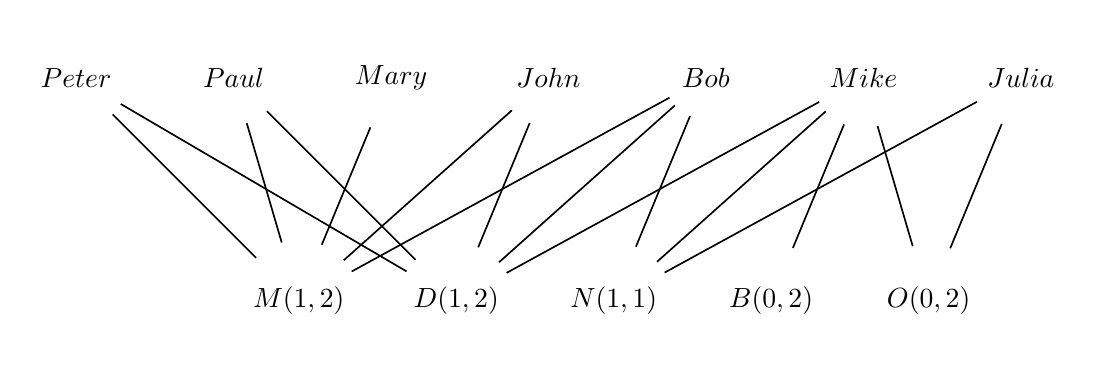
\begin{tikzpicture}[-,>=stealth',shorten >=1pt,auto,node distance=2cm,
                    semithick]
  \tikzstyle{every state}=[fill=white,draw=none,text=black]

  \node[state]         (PETER)                  {$Peter$};
  \node[state]         (PAUL) [right of=PETER]  {$Paul$};
  \node[state]         (MARY) [right of=PAUL]   {$Mary$};
  \node[state]         (JOHN) [right of=MARY]   {$John$};
  \node[state]         (BOB)  [right of=JOHN]   {$Bob$};
  \node[state]         (MIKE) [right of=BOB]    {$Mike$};
  \node[state]         (JULIA)[right of=MIKE]   {$Julia$};
  \node[state]         (NONE)[below right of=PETER] {$ $};
  \node[state]         (M)[below right of=NONE]{$M(1,2)$};
  \node[state]         (D)[right of=M]          {$D(1,2)$};
  \node[state]         (N)[right of=D]          {$N(1,1)$};
  \node[state]         (B)[right of=N]          {$B(0,2)$};
  \node[state]         (O)[right of=B]          {$O(0,2)$};

  \path (M) edge node {} (PETER)
            edge node {} (PAUL)
            edge node {} (MARY)
            edge node {} (JOHN)
            edge node {} (BOB)
        (D) edge node {} (PETER)
            edge node {} (PAUL)
            edge node {} (JOHN)
            edge node {} (BOB)
            edge node {} (MIKE)
        (N) edge node {} (BOB)
            edge node {} (MIKE)
            edge node {} (JULIA)
        (B) edge node {} (MIKE)
        (O) edge node {} (MIKE)
            edge node {} (JULIA);
\end{tikzpicture}}
\end{center}

On peut assigner $Bob$ à la tache $N$ et assigner à $Julia$ la tache $O$, le reste sera des combinaison possible:
\begin{center} \scalebox{0.8}{
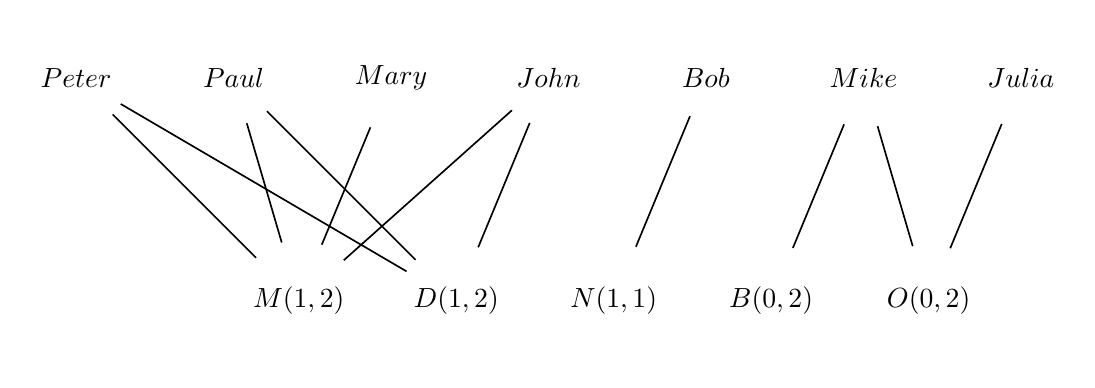
\begin{tikzpicture}[-,>=stealth',shorten >=1pt,auto,node distance=2cm,
                    semithick]
  \tikzstyle{every state}=[fill=white,draw=none,text=black]

  \node[state]         (PETER)                  {$Peter$};
  \node[state]         (PAUL) [right of=PETER]  {$Paul$};
  \node[state]         (MARY) [right of=PAUL]   {$Mary$};
  \node[state]         (JOHN) [right of=MARY]   {$John$};
  \node[state]         (BOB)  [right of=JOHN]   {$Bob$};
  \node[state]         (MIKE) [right of=BOB]    {$Mike$};
  \node[state]         (JULIA)[right of=MIKE]   {$Julia$};
  \node[state]         (NONE)[below right of=PETER] {$ $};
  \node[state]         (M)[below right of=NONE]{$M(1,2)$};
  \node[state]         (D)[right of=M]          {$D(1,2)$};
  \node[state]         (N)[right of=D]          {$N(1,1)$};
  \node[state]         (B)[right of=N]          {$B(0,2)$};
  \node[state]         (O)[right of=B]          {$O(0,2)$};

  \path (M) edge node {} (PETER)
            edge node {} (PAUL)
            edge node {} (MARY)
            edge node {} (JOHN)
        (D) edge node {} (PETER)
            edge node {} (PAUL)
            edge node {} (JOHN)
        (N) edge node {} (BOB)
        (B) edge node {} (MIKE)
        (O) edge node {} (MIKE)
            edge node {} (JULIA);
\end{tikzpicture}}
\end{center}

\section{AC filtre Sum à une borne}

Soit un filtre $sum$ avec les variables $(x,y,z,a,b,c)$ dans le domaine $range(1,5)$ appliqué sur l'équation:
\formula{$2x+3y+2z+a+4b+2c \geq 50$}
\begin{center}
\begin{tabular}{cccccc}
x&y&z&a&b&c\\ \hline
1&1&1&1&1&1\\ 2&2&2&2&2&2\\ 3&3&3&3&3&3\\ 4&4&4&4&4&4\\
\end{tabular}
\end{center}
Si le somme des maximums de chaque variable ne respecte pas la contrainte, alors il n'existe aucun assignement des variables tel que la contrainte serait satisfaite:
\formula{$2*4+3*4+2*4+4+4*4+2*4 = 8+12+8+4+16+8 = 56 \geq 50$}
Pour chaque variables, enlever son impacte dans le résultat précédemment obtenue et refaire l'opération de dépilé avec les différents $x$ tant que un $x_i$ ne satisfait pas la contrainte:\\
\ \\
Pour x:
\begin{description}
\item[] $2*4+3*4+2*4+4+4*4+2*4 = 8+12+8+4+16+8 = 56 \geq 50$
\item[] $ 56 - 2*4 + 2*1 = 50 \geq 50$, donc $x=1$ fonctionne
\item[] (pareil pour z,c)
\end{description}
\ \\
Pour y:
\begin{description}
\item[] $ 56 - 3*4 + 3*1 = 44 \geq 50$, donc $y=1$  ne fonctionne pas
\item[] $ 56 - 3*4 + 3*2 = 50 \geq 50$, donc $y=2$  fonctionne
\end{description}
\pagebreak
Pour b:
\begin{description}
\item[] $ 56 - 4*4 + 4*1 = 40 \geq 50$, donc $b=1$  ne fonctionne pas
\item[] $ 56 - 4*4 + 4*2 = 44 \geq 50$, donc $b=2$  ne fonctionne pas
\item[] $ 56 - 4*4 + 4*3 = 50 \geq 50$, donc $b=3$  fonctionne
\end{description}
\ \\
On obtient:\\
\begin{center}
\begin{tabular}{cccccc}
x&y&z&a&b&c\\ \hline
1&$ $&1&1&$ $&1\\ 2&2&2&2&$ $&2\\ 3&3&3&3&3&3\\ 4&4&4&4&4&4\\
\end{tabular}
\end{center}

\pagebreak
\section{AC filtre avec Sum à deux bornes}

\begin{multicols}{3}
[Soit $x,y,z$ avec comme domaine $dom(x)=dom(y)=dom(z) = {1,2}$ et avec une contrainte $8 \leq 2x + 2y + z \leq 9$.\\
Via résolution graphique on obtient et réduit le graphe comme ceci:]

\scalebox{0.8}{
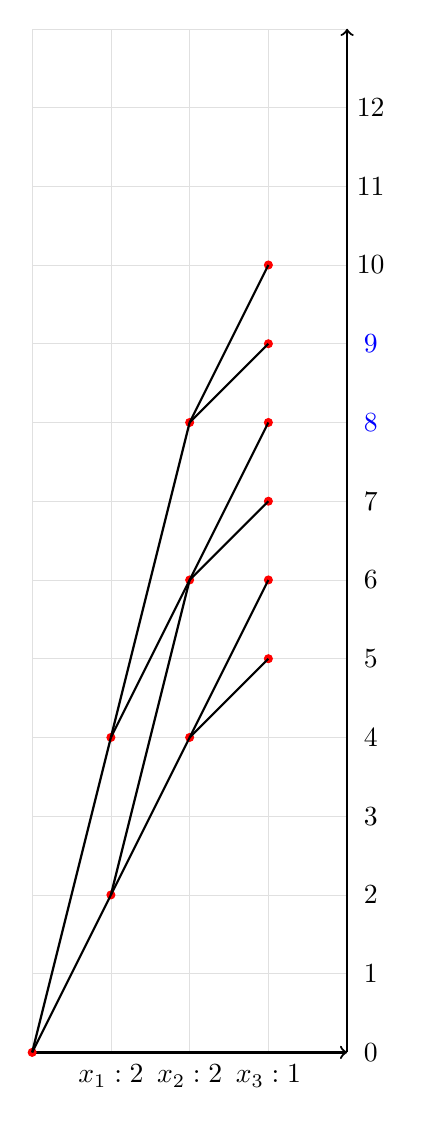
\begin{tikzpicture}
 \draw[help lines, gray!20] (0,0) grid (4,13);
 
 \node at (1,-0.3) {$x_1:2$};
 \node at (2,-0.3) {$x_2:2$};
 \node at (3,-0.3) {$x_3:1$};

 \draw [->, thick] (0,0) -- (4,0);
 \draw [->, thick] (4,0) -- (4,13);
 
 \foreach \vec in {0,1,2,3,4,5,6,7,10,11,12}{
 	\node at (4.3,\vec) {$\vec$};
 }
 
  \foreach \vec in {8,9}{
 	\node at (4.3,\vec) {$\cblue{\vec}$};
 }
 
 \foreach \vec in {(0,0),(1,2),(1,4),(2,4),(2,6),(2,8),(3,5),(3,6),(3,7),(3,8),(3,9),(3,10)}{
 	\draw [fill, red] \vec circle [radius=0.05];
 }
 
 \draw [thick, black] (0,0) -- (1,2);
 \draw [thick, black] (0,0) -- (1,4);
 \draw [thick, black] (1,2) -- (2,4);
 \draw [thick, black] (1,2) -- (2,6);
 \draw [thick, black] (1,4) -- (2,6);
 \draw [thick, black] (1,4) -- (2,8);
 \draw [thick, black] (2,4) -- (3,5);
 \draw [thick, black] (2,4) -- (3,6);
 \draw [thick, black] (2,6) -- (3,7);
 \draw [thick, black] (2,6) -- (3,8);
 \draw [thick, black] (2,8) -- (3,9);
 \draw [thick, black] (2,8) -- (3,10);
 
\end{tikzpicture}}

\scalebox{0.8}{
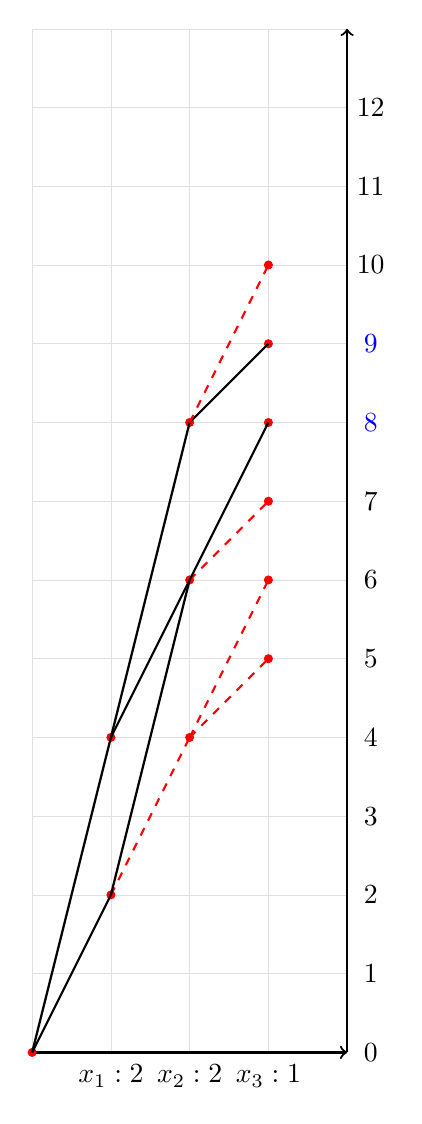
\begin{tikzpicture}
 \draw[help lines, gray!20] (0,0) grid (4,13);
 
 \node at (1,-0.3) {$x_1:2$};
 \node at (2,-0.3) {$x_2:2$};
 \node at (3,-0.3) {$x_3:1$};

 \draw [->, thick] (0,0) -- (4,0);
 \draw [->, thick] (4,0) -- (4,13);
 
 \foreach \vec in {0,1,2,3,4,5,6,7,10,11,12}{
 	\node at (4.3,\vec) {$\vec$};
 }
 
  \foreach \vec in {8,9}{
 	\node at (4.3,\vec) {$\cblue{\vec}$};
 }
 
 \foreach \vec in {(0,0),(1,2),(1,4),(2,4),(2,6),(2,8),(3,5),(3,6),(3,7),(3,8),(3,9),(3,10)}{
 	\draw [fill, red] \vec circle [radius=0.05];
 }
 
 \draw [thick, black] (0,0) -- (1,2);
 \draw [thick, black] (0,0) -- (1,4);
 \draw [thick, dashed, red] (1,2) -- (2,4);
 \draw [thick, black] (1,2) -- (2,6);
 \draw [thick, black] (1,4) -- (2,6);
 \draw [thick, black] (1,4) -- (2,8);
 \draw [thick, dashed, red] (2,4) -- (3,5);
 \draw [thick, dashed, red] (2,4) -- (3,6);
 \draw [thick, dashed, red] (2,6) -- (3,7);
 \draw [thick, black] (2,6) -- (3,8);
 \draw [thick, black] (2,8) -- (3,9);
 \draw [thick, dashed, red] (2,8) -- (3,10);
 
\end{tikzpicture}}

\scalebox{0.8}{
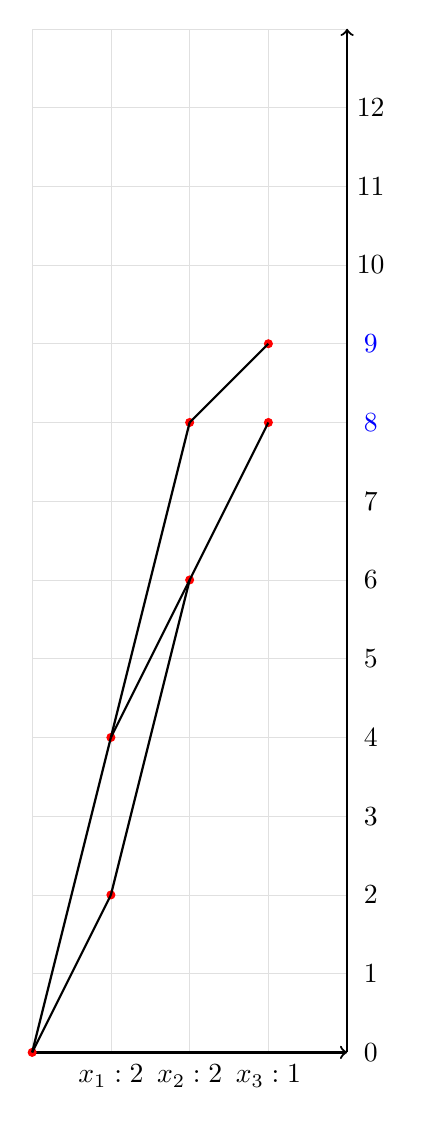
\begin{tikzpicture}
 \draw[help lines, gray!20] (0,0) grid (4,13);
 
 \node at (1,-0.3) {$x_1:2$};
 \node at (2,-0.3) {$x_2:2$};
 \node at (3,-0.3) {$x_3:1$};

 \draw [->, thick] (0,0) -- (4,0);
 \draw [->, thick] (4,0) -- (4,13);
 
 \foreach \vec in {0,1,2,3,4,5,6,7,10,11,12}{
 	\node at (4.3,\vec) {$\vec$};
 }
 
  \foreach \vec in {8,9}{
 	\node at (4.3,\vec) {$\cblue{\vec}$};
 }
 
 \foreach \vec in {(0,0),(1,2),(1,4),(2,6),(2,8),(3,8),(3,9)}{
 	\draw [fill, red] \vec circle [radius=0.05];
 }
 
 \draw [thick, black] (0,0) -- (1,2);
 \draw [thick, black] (0,0) -- (1,4);
 \draw [thick, black] (1,2) -- (2,6);
 \draw [thick, black] (1,4) -- (2,6);
 \draw [thick, black] (1,4) -- (2,8);
 \draw [thick, black] (2,6) -- (3,8);
 \draw [thick, black] (2,8) -- (3,9);
 
\end{tikzpicture}}
\end{multicols}

Dans un premier temps on représente toutes les possibilités, dans un second temps on élimine récursivement tout les feuille de l'arbre qui pointe sur des noeuds hors objectif (dans notre cas hors de 8,9). Toutes les branches seul qui ne sont pas relié aux bornes 8 et 9 seront supprimé.\\
On peut attribuer au variables toutes les possibilités de chemin de l'arbre:
\begin{description}
\item[] $x_1=1, x_2=2, x_3=1$ : $1*2 + 2*2 + 1*2 = 8$
\item[] $x_1=2, x_2=2, x_3=1$ : $2*2 + 2*2 + 1*1 = 9$
\end{description}
\pagebreak

\chapter{Recherche de réponses}
Selon les problèmes, l'arbre de décision peut être assez profond / large à explorer, on peut inféré sur les contraintes par filtrage ou par propagation pour ne pas à avoir à explorer certains sous arbres.
\pagebreak

\section{recherche avec backtrack}
Tout dépend du niveau de l'algorithme de filtrage utilisé, en utilisant $look-ahead$ algorithme on obtient:
\begin{description}
\item[BT] $ $
\item[FC] (Forward Checking)
\item[MAC] (Maintaining Arc Consistency)
\end{description}

Pour l'algorithme $look-back$ effectuant des choses plus intelligente:
\begin{description}
\item[CBJ] (Conflict-directed backjumping)
\item[DBT] (Dynamic Backtracking)
\end{description}

\pagebreak
\subsection{BT}
BT est le plus simple, pour chaque node, on va regarder si celui ci satisfait toutes les contraintes.
Sur le problème des N-queens=4:
\begin{multicols}{3}
\scalebox{0.9}{
\begin{tabular}{c|c|c|c}
$ $&$X$&$ $&$ $\\\hline
$ $&$ $&$ $&$ $\\\hline
$ $&$ $&$ $&$ $\\\hline
$X$&$ $&$ $&$ $\\
\end{tabular}
}
\scalebox{0.9}{
\begin{tabular}{c|c|c|c}
$ $&$X$&$ $&$ $\\\hline
$ $&$ $&$ $&$ $\\\hline
$ $&$ $&$ $&$ $\\\hline
$\crouge{X}$&$ $&$\crouge{X}$&$ $\\
\end{tabular}
}
\scalebox{0.9}{
\begin{tabular}{c|c|c|c}
$ $&$X$&$ $&$ $\\\hline
$ $&$ $&$ $&$ $\\\hline
$ $&$ $&$X$&$ $\\\hline
$X$&$ $&$ $&$ $\\
\end{tabular}
}
\end{multicols}

\begin{multicols}{3}
\scalebox{0.9}{
\begin{tabular}{c|c|c|c}
$ $&$X$&$ $&$ $\\\hline
$ $&$ $&$ $&$ $\\\hline
$ $&$ $&$X$&$ $\\\hline
$\crouge{X}$&$ $&$ $&$\crouge{X}$\\
\end{tabular}
}
\scalebox{0.9}{
\begin{tabular}{c|c|c|c}
$ $&$X$&$ $&$ $\\\hline
$ $&$ $&$ $&$ $\\\hline
$ $&$ $&$\crouge{X}$&$\crouge{X}$\\\hline
$X$&$ $&$ $&$ $\\
\end{tabular}
}
\scalebox{0.9}{
\begin{tabular}{c|c|c|c}
$ $&$X$&$ $&$ $\\\hline
$ $&$ $&$ $&$\crouge{X}$\\\hline
$ $&$ $&$\crouge{X}$&$ $\\\hline
$X$&$ $&$ $&$ $\\
\end{tabular}
}
\end{multicols}

\begin{multicols}{3}
\scalebox{0.9}{
\begin{tabular}{c|c|c|c}
$ $&$X$&$ $&$\crouge{X}$\\\hline
$ $&$ $&$ $&$ $\\\hline
$ $&$ $&$X$&$ $\\\hline
$\crouge{X}$&$ $&$ $&$ $\\
\end{tabular}
}
\scalebox{0.9}{
\begin{tabular}{c|c|c|c}
$ $&$X$&$ $&$ $\\\hline
$ $&$ $&$\crouge{X}$&$ $\\\hline
$ $&$ $&$ $&$ $\\\hline
$\crouge{X}$&$ $&$ $&$ $\\
\end{tabular}
}
\scalebox{0.9}{
\begin{tabular}{c|c|c|c}
$ $&$\crouge{X}$&$\crouge{X}$&$ $\\\hline
$ $&$ $&$ $&$ $\\\hline
$ $&$ $&$ $&$ $\\\hline
$X$&$ $&$ $&$ $\\
\end{tabular}
}
\end{multicols}

\begin{multicols}{3}
\scalebox{0.9}{
\begin{tabular}{c|c|c|c}
$ $&$ $&$ $&$ $\\\hline
$ $&$ $&$ $&$ $\\\hline
$X$&$ $&$ $&$ $\\\hline
$ $&$ $&$ $&$ $\\
\end{tabular}
}
\scalebox{0.9}{
\begin{tabular}{c|c|c|c}
$ $&$ $&$ $&$ $\\\hline
$ $&$ $&$ $&$ $\\\hline
$\crouge{X}$&$ $&$ $&$ $\\\hline
$ $&$\crouge{X}$&$ $&$ $\\
\end{tabular}
}
\scalebox{0.9}{
\begin{tabular}{c|c|c|c}
$ $&$ $&$ $&$ $\\\hline
$ $&$ $&$ $&$ $\\\hline
$\crouge{X}$&$\crouge{X}$&$ $&$ $\\\hline
$ $&$ $&$ $&$ $\\
\end{tabular}
}
\end{multicols}
\pagebreak

\subsection{FC}
FC, toutes les nodes utilisé réduire le domaine des autres nodes, si un domaine est vide, plus besoin de continuer il n'y a pas de solution:
Sur le problème des N-queens=4:
\begin{multicols}{3}
\scalebox{0.9}{
\begin{tabular}{c|c|c|c}
$ $&$ $&$ $&$\crouge{\#}$\\\hline
$ $&$ $&$\crouge{\#}$&$ $\\\hline
$ $&$\crouge{\#}$&$ $&$ $\\\hline
$X$&$\crouge{\#}$&$\crouge{\#}$&$\crouge{\#}$\\
\end{tabular}
}
\scalebox{0.9}{
\begin{tabular}{c|c|c|c}
$ $&$ $&$\crouge{\#}$&$\crouge{\#}$\\\hline
$ $&$X$&$\crouge{\#}$&$\crouge{\#}$\\\hline
$ $&$\crouge{\#}$&$ $&$ $\\\hline
$X$&$\crouge{\#}$&$\crouge{\#}$&$\crouge{\#}$\\
\end{tabular}
}
\scalebox{0.9}{
\begin{tabular}{c|c|c|c}
$ $&$ $&$ $&$\crouge{\#}$\\\hline
$ $&$\crouge{\#}$&$\crouge{\#}$&$ $\\\hline
$ $&$\crouge{\#}$&$ $&$ $\\\hline
$X$&$\crouge{\#}$&$\crouge{\#}$&$\crouge{\#}$\\
\end{tabular}
}
\end{multicols}

\begin{multicols}{3}
\scalebox{0.9}{
\begin{tabular}{c|c|c|c}
$ $&$X$&$\crouge{\#}$&$\crouge{\#}$\\\hline
$ $&$\crouge{\#}$&$\crouge{\#}$&$ $\\\hline
$ $&$\crouge{\#}$&$ $&$\crouge{\#}$\\\hline
$X$&$\crouge{\#}$&$\crouge{\#}$&$\crouge{\#}$\\
\end{tabular}
}
\scalebox{0.9}{
\begin{tabular}{c|c|c|c}
$ $&$X$&$\crouge{\#}$&$\crouge{\#}$\\\hline
$ $&$\crouge{\#}$&$\crouge{\#}$&$\crouge{\#}$\\\hline
$ $&$\crouge{\#}$&$X$&$\crouge{\#}$\\\hline
$X$&$\crouge{\#}$&$\crouge{\#}$&$\crouge{\#}$\\
\end{tabular}
}
\scalebox{0.9}{
\begin{tabular}{c|c|c|c}
$ $&$X$&$\crouge{\#}$&$\crouge{\#}$\\\hline
$ $&$\crouge{\#}$&$\crouge{\#}$&$ $\\\hline
$ $&$\crouge{\#}$&$X$&$\crouge{\#}$\\\hline
$X$&$\crouge{\#}$&$\crouge{\#}$&$\crouge{\#}$\\
\end{tabular}
}
\end{multicols}

\begin{multicols}{3}
\scalebox{0.9}{
\begin{tabular}{c|c|c|c}
$ $&$\crouge{\#}$&$ $&$\crouge{\#}$\\\hline
$ $&$\crouge{\#}$&$\crouge{\#}$&$ $\\\hline
$ $&$\crouge{\#}$&$ $&$ $\\\hline
$X$&$\crouge{\#}$&$\crouge{\#}$&$\crouge{\#}$\\
\end{tabular}
}
\scalebox{0.9}{
\begin{tabular}{c|c|c|c}
$ $&$ $&$ $&$\crouge{\#}$\\\hline
$ $&$ $&$\crouge{\#}$&$ $\\\hline
$X$&$\crouge{\#}$&$\crouge{\#}$&$\crouge{\#}$\\\hline
$\crouge{\#}$&$ $&$ $&$ $\\
\end{tabular}
}
\scalebox{0.9}{
\begin{tabular}{c|c|c|c}
$ $&$X$&$\crouge{\#}$&$\crouge{\#}$\\\hline
$ $&$\crouge{\#}$&$\crouge{\#}$&$ $\\\hline
$X$&$\crouge{\#}$&$\crouge{\#}$&$\crouge{\#}$\\\hline
$\crouge{\#}$&$ $&$ $&$ $\\
\end{tabular}
}
\end{multicols}

\begin{multicols}{3}
\scalebox{0.9}{
\begin{tabular}{c|c|c|c}
$ $&$X$&$\crouge{\#}$&$\crouge{\#}$\\\hline
$ $&$\crouge{\#}$&$\crouge{\#}$&$ $\\\hline
$X$&$\crouge{\#}$&$\crouge{\#}$&$\crouge{\#}$\\\hline
$\crouge{\#}$&$ $&$X$&$ $\\
\end{tabular}
}
\scalebox{0.9}{
\begin{tabular}{c|c|c|c}
$ $&$X$&$\crouge{\#}$&$\crouge{\#}$\\\hline
$ $&$\crouge{\#}$&$\crouge{\#}$&$X$\\\hline
$X$&$\crouge{\#}$&$\crouge{\#}$&$\crouge{\#}$\\\hline
$\crouge{\#}$&$ $&$X$&$ $\\
\end{tabular}
}
\scalebox{0.9}{
\begin{tabular}{c|c|c|c}
$ $&$X$&$ $&$ $\\\hline
$ $&$ $&$ $&$X$\\\hline
$X$&$ $&$ $&$ $\\\hline
$ $&$ $&$X$&$ $\\
\end{tabular}
}
\end{multicols}
\pagebreak
\subsection{MAC binary AC search}

%% fill

\subsection{CBJ}

%% fill

\section{Heuristiques de recherche}

%% fill

\pagebreak
\part{Problème de satisfaction SAT}
\pagebreak

\chapter{définitions de base}
\pagebreak

\section{Transformation NNF, CNF}

Une forme NNF (Negative Normal Forme) est une formule donné avec uniquement les connecteurs logique $\wedge \vee \neg$.\\

\begin{description}
\item[] en remplaçant les $\rightarrow$ et $\leftrightarrow$: \begin{description}
\item[] $\phi \rightarrow \psi$ donne $\neg \phi \vee \psi$
\item[] $\phi \leftrightarrow \psi$ donne $(\neg \phi \vee \psi) \wedge ( \phi \vee \neg \psi)$
\end{description}
\item[] descendre les négations au niveau atomique: \begin{description}
\item[] $\neg (\phi \wedge \psi)$ donne $\neg \phi \vee \neg \psi$
\item[] $\neg (\phi \vee \psi)$ donne $\neg \phi \wedge \neg \psi$
\item[] $\neg \neg \phi$ donne $\phi$
\end{description}
\end{description}

Une forme CNF (Normal Conjonctive Forme) est une conjonction de disjonctions de littéraux:
\begin{description}
\item[exemple]: $(\neg A \vee B) \wedge (\neg C \vee B \vee D) \wedge (A \vee B)$
\end{description}

\subsection{Transformation glouton}

Toutes formules peut être réduite à CNF en appliquant récursivement la lois de DeMorgan:
\begin{description}
\item[] $(\phi \wedge \psi) \vee \gamma$ donne $(\phi \vee \gamma) \wedge (\psi \vee \gamma)$
\end{description}

Mais rarement utilisé car la complexité est exponentielle dans le pire des cas.\\

\pagebreak
\subsection{Transformation via ajout de variables}

Soit la formule suivante:
\begin{description}
\item[] $\neg((\neg(a \vee b)) \leftrightarrow ( c\rightarrow d))\rightarrow((e1\wedge e2\wedge e3) \vee (f1 \wedge f2 \wedge f3)\vee (g1 \wedge g2 \wedge g3))$
\end{description}

réduire en NNF:

\begin{description}
\item[] $((a \vee b \vee \neg c \vee d) \wedge ((c \wedge \neg d) \vee (\neg a \wedge \neg b)) \vee ((e1 \wedge e2 \wedge e3) \vee (f1 \wedge f2 \wedge f3)\vee(g1 \wedge g2 \wedge g3))$
\end{description}

Appliquer la formule:\\
$((a \vee b \vee \neg c \vee d) \wedge (\crouge{(c \wedge \neg d)} \vee \cblue{(\neg a \wedge \neg b)}) \vee (\corange{(e1 \wedge e2 \wedge e3)} \vee \cviolet{(f1 \wedge f2 \wedge f3)}\vee \cvert{(g1 \wedge g2 \wedge g3)})$\\

\begin{description}
\item[$\crouge{i}$] $\leftrightarrow \crouge{(c \wedge \neg d)}$
\item[$\cblue{j}$] $\leftrightarrow \cblue{(\neg a \wedge \neg b)}$
\item[$\corange{k}$] $\leftrightarrow \corange{(e1 \wedge e2 \wedge e3)}$
\item[$\cviolet{l}$] $\leftrightarrow \cviolet{(f1 \wedge f2 \wedge f3)}$
\item[$\cvert{m}$] $\leftrightarrow \cvert{(g1 \wedge g2 \wedge g3)}$
\end{description}

donne:\\
$(\cgris{(a \vee b \vee \neg c \vee d) \wedge (\crouge{i} \vee \cblue{j})} \vee (\corange{k} \vee \cviolet{l}\vee \cvert{m})$\\

\begin{description}
\item[$\cgris{n}$] $\leftrightarrow \cgris{(a \vee b \vee \neg c \vee d) \wedge (\crouge{i} \vee \cblue{j})}$
\end{description}

ce qui donne:\\
$(\cgris{n} \vee \corange{k} \vee \cviolet{l}\vee \cvert{m})$\\

\pagebreak
\ \\
Après distribution des nouvelles variables:\\
\ \\
$(\cgris{n} \vee \corange{k} \vee \cviolet{l}\vee \cvert{m}) \wedge $\\
$\crouge{i} \leftrightarrow \crouge{(c \wedge \neg d)} \wedge $\\ 
$\cblue{j} \leftrightarrow \cblue{(\neg a \wedge \neg b)} \wedge $\\
$\corange{k} \leftrightarrow \corange{(e1 \wedge e2 \wedge e3)} \wedge $\\
$\cviolet{l} \leftrightarrow \cviolet{(f1 \wedge f2 \wedge f3)} \wedge $\\
$\cvert{m} \leftrightarrow \cvert{(g1 \wedge g2 \wedge g3)} \wedge $\\
$\cgris{n} \leftrightarrow \cgris{(a \vee b \vee \neg c \vee d) \wedge (\crouge{i} \vee \cblue{j}})$
\\

donne la formule CNF suivante:\\
$((n \vee k \vee l \vee m)\wedge (\neg i \vee c)\wedge (\neg i \vee \neg d)\wedge$\\
$(\neg j \vee \neg a)\wedge(\neg j \vee \neg b)\wedge(\neg k \vee e1)\wedge(\neg k \vee e2)\wedge(\neg k \vee e3)\wedge$\\
$(\neg l \vee f1)\wedge(\neg l \vee f2)\wedge\neg l \vee f3)\wedge(\neg m \vee g1)\wedge(\neg m \vee g2)\wedge\neg m \vee g3)\wedge$\\
$(\neg n \vee a \vee b \vee \neg c \ vee d)\wedge(\neg n \vee i \vee j)$\\

\section{Littéral et clause : classification}

Soit la formule suivante avec les littéraux de couleur vert des littéraux équivalent à $\top$ et en bleu les littéraux équivalent à $\bot$:\\
\formula{$(\cblue{a} \vee \cblue{\neg b}) \wedge (\cvert{\neg a} \vee \cvert{b} \vee \neg c) \wedge (\cblue{a} \vee c \vee d)$}

Via déduction la clause:
\begin{description}
\item[] $(\cblue{a} \vee \cblue{\neg b})$ est falsifié
\item[] $(\cvert{\neg a} \vee \cvert{b} \vee \neg c)$ est satisfaite
\item[] $(\cblue{a} \vee c \vee d)$ est active
\end{description}

\pagebreak
\subsection{Clause active}
Une clause active est unitaire si elle a exactement un littéral non affecté:
\begin{description}
\item[] $(\cvert{a} \vee c) \wedge (\cvert{b} \vee c) \wedge (\blue{\neg a} \vee \cblue{\neg b} \vee \neg c)$
\item[] est I une interprétation tel que I(a) = $\top$ et I(b) = $\bot$.
\end{description}
Dans ce cas, une cause unitaire admet qu'une seul solution pour être satisfaite:
\formula{$a \wedge b \rightarrow \neg c$}
$c$ doit être affecté à $\top$.\\

\subsection{Littéral pure}
Une variable est dite pure dans une formule si ses littéraux sont soit tous positif ou tous négatifs:\\
\formula{$(a \vee \cblue{c}) \wedge (\neg a \vee \cblue{c})$}
\pagebreak

\chapter{Classes polynomiales}
\pagebreak
\section{2-SAT}
Une formule sous forme 2-SAT est une formule où chaque termes de la formule est binaire.
La résolution est en temps polynomiale.\\


\section{Horn-SAT}
Une clause est dite de Horn si elle contient au plus un littéral positif:
\begin{description}
\item[] $(a) \rightarrow a$ 
\item[] $(a \vee \neg b \vee \neg c) \rightarrow a :- b, c$
\item[] $(\neg a \vee \neg b \vee \neg c) \rightarrow :- a, b, c$
\end{description}

\section{Horn-renommable}
Une formule est Horn renommable si une fois avoir appliquer l'inverser sur tout les littéraux d'une formule, celle ci devient Horn-SAT:\\
\begin{description}
\item[$\phi$] = $(\neg a \vee b) \wedge (a \vee b \vee c)$
\item[$H(\phi)$] = $(a \vee \neg b) \wedge (\neg a \vee \neg b \vee \neg c)$
\end{description}

\pagebreak

\chapter{Algorithmes de résolution syntaxiques}
\pagebreak
\section{Algorithmes complets basé sur la résolution}
\subsection{Méthodes basé sur la résolution}

Soit une règles de résolution:
\formula{$\frac{w_1 = (\neg a \vee \alpha) \wedge (w_2 = (a \vee \beta)}{(r = (\alpha \vee \beta)}$}

On n'a $w_1 \wedge w_2 \models r$ car via affectation de la valeur de $a$ on retrouve bien $r$.\\

\subsection{Modus Ponuce}

% fill

\subsection{règles de subsumption}

Soit:
\formula{$(w_1 = (a \vee b)) et (w_2 = (a \vee b \vee c))$}

On peut dire que $w_1 \models w_2$.

\subsection{Règles de fusion}

% fill

\section{Algorithmes complets Procédure de Davis et Putnam}

Prend que des formules CNF.\\

$Tant que(\bot \neg \in) et (\top \neg \in \sigma) faire:$
\begin{description}
\item[] appliquer la règles de littéraux unitaires
\item[] appliquer la règles de littéraux pures
\item[] choisir une variable $p \in Atomes(\sigma)$ et construire une nouvelle formule $\sigma = \sigma sans p$
\end{description}

Soit:
\formula{$(a \vee c) (b \vee c) (d \vee c) (\neg a \vee \neg b \vee \neg c)$}
Appliquer la règles de littéraux unitaires:
\formula{$(a \vee c) (b \vee c) (d \vee c) (\neg a \vee \neg b \vee \neg c)$}
Appliquer la règles de littéraux pures
\formula{$(a \vee c) (b \vee c) \crouge{(d \vee c)} (\neg a \vee \neg b \vee \neg c)$}
\formula{$(a \vee c) (b \vee c) (\neg a \vee \neg b \vee \neg c)$}
Éliminer la variable c
\formula{$(a \vee \neg a \vee \neg b) (b \vee \neg a \vee \neg b) = \top$}

Rarement utilisé en pratique.

\section{Algorithmes complets Méthodes des tableaux}

Prend n'importe quel type de formules:\\
Voir cours de Représentation des connaissances et raisonnement.\\

\chapter{Algorithmes de résolutions avec backtraking}

\section{Procédure de DPLL}

% fill
% only cnf
% si unitaire ou pure : résoudre
% sinon faire 2 branches d'affectations sur une var

\chapter{Solveurs SAT modernes}
\pagebreak

\chapter{Algorithmes incomplets}

\section{GSAT recherche locale}

Partir d'une formule où tout les littéraux sont affecté aléatoirement à $\top$ ou $\bot$ puis pour un nombre d'itération donné si la formule n'est pas satisfiable alors prendre un terme aléatoirement et l'inverser.\\

\section{Tabou pour Sat}

Une amélioration de GSAT et d'utiliser une File, inverser un littéral c'est l'enfiler dans le File, une fois dans le File ce littéral de peut plus être inversé, au bout de n tours, le littéral en File est enlevé.\\
Lors d'un 3-SAT le nombre n de tours est optimisé si il veut le nombre de variables de la formule\\

\pagebreak
\chapter{Méthodes mixtes ROBDD, OBDD, BDD}
\pagebreak

\section{BDD}
Tout formule peut être reproduit sous forme INF ($if\ then\ else\ normal\ forme$), soi l'opérateur $if-then-else (ite)$:
\formula{$x \hookrightarrow y, z = (x \wedge y) \vee (\neg x \wedge z)$}
\begin{description}
\item[] $\neg x$ par $x \hookrightarrow 0,1$
\item[] $x \Rightarrow y$ par $x \hookrightarrow (y \hookrightarrow 1, 0), 1$
\item[] $x \Leftrightarrow y$ par $x \hookrightarrow (y \hookrightarrow 1,0), (y \hookrightarrow 0,1)$
\item[] $x \wedge y$ par  $x \hookrightarrow (y \hookrightarrow 1, 0), 0$
\item[] $x \vee y$ par $x \hookrightarrow 1, (y \hookrightarrow 1,0)$
\end{description}

Soit la formule suivante:
\formula{$\phi = (x_1 \Leftrightarrow y_1) \wedge (x_2 \Leftrightarrow y_2)$}
\begin{multicols}{2}
[En appliquant récursivement le théorème de Shanon sur les variables (mises dans un ordre) on obtient:]
\begin{description}
\item[$\phi$] = $x_1 \hookrightarrow \phi_1, \phi_0$
\item[$\phi_0$] = $y_1 \hookrightarrow 0, \phi_{00}$
\item[$\phi_1$] = $y_1 \hookrightarrow \phi_{11}, 0$
\item[$\phi_{00}$] = $x_2 \hookrightarrow \phi_{001}, \phi_{000}$
\item[$\phi_{11}$] = $x_2 \hookrightarrow \phi_{111}, \phi_{110}$
\item[$\phi_{000}$] = $y_2 \hookrightarrow 0, 1$
\item[$\phi_{001}$] = $y_2 \hookrightarrow 1, 0$
\item[$\phi_{110}$] = $y_2 \hookrightarrow 0, 1$
\item[$\phi_{111}$] = $y_2 \hookrightarrow 1, 0$
\end{description}

\begin{tikzpicture}[
  level distance=15mm,
  text depth=.1em,
  text height=.8em,
  level 1/.style={sibling distance=8em},
  level 2/.style={sibling distance=4em},
  level 3/.style={sibling distance=4em},
  level 4/.style={sibling distance=2em},
  every node/.style = {scale=1,
    draw=none, align=center}]]
  \node {$x_1$}
    child { node {$y_1$} 
      child { node {$x_2$}
        child { node {$y_2$ }
            child { node {$\top$ }}
        	child { node {$\bot$ }}
        }
        child { node {$y_2$ }
            child { node {$\bot$ }}
        	child { node {$\top$ }}
        }
      }
      child { node {$\bot$}
      }
    }
    child { node {$y_1$} 
      child { node {$\bot$}
      }
      child { node {$x_2$}
        child { node {$y_2$ }
            child { node {$\top$ }}
        	child { node {$\bot$ }}
        }
        child { node {$y_2$ }
            child { node {$\bot$ }}
        	child { node {$\top$ }}
        }
      }
    };
\end{tikzpicture}
\end{multicols}

\pagebreak
Vers un ROBDD, la simplification se fait en fusionnant les noeuds ayant le même parent, et en instance que 2 feuilles ($\top$ et $\bot$):

\scalebox{0.7}{
\begin{tikzpicture}[->,>=stealth',shorten >=1pt,auto,node distance=4cm,
                    semithick]
  \tikzstyle{every state}=[fill=white,draw=none,text=black]

  \node[state]         (x1) [] {$x_1$};
  \node[state]         (y1t) [below left of=x1] {$y_1$};
  \node[state]         (y1f) [below right of=x1] {$y_1$};
  \node[state]         (x2) [below of=y1t] {$x_2$};
  \node[state]         (y2t) [below right of=x2] {$y_2$};
  \node[state]         (y2f) [below left of=x2] {$y_2$};
  \node[state]         (r0) [below left of=y2f] {$0$};
  \node[state]         (r1) [below left of=y2t] {$1$};

  \path (y1t) edge              node {} (x1)
  		(y1f) edge node {} (x1)
  		(x2) edge node {} (y1f)
  		 edge node {} (y1t)
  		 (y2f) edge node {} (x2)
  		 (y2t) edge node {} (x2)
  		 (r0) edge node {} (y1f)
  		 edge node {} (y2t)
  		 (r1) edge node {} (y2f)
  		 edge node {} (y2t);
\end{tikzpicture}
}



\pagebreak
\pagebreak
\pagebreak
\end{document}

